% ============================================================================
% Quantized Inertia under Covariant and Quantum-Field-Theoretic Audit
% Framework-independent manuscript
% Copyright (c) 2026 Henry Arellano-Pena - CC BY 4.0
% ============================================================================

\documentclass[11pt]{article}

\usepackage[margin=1in]{geometry}
\usepackage[T1]{fontenc}
\usepackage[utf8]{inputenc}
\usepackage{lmodern}
\usepackage{microtype}
\usepackage{setspace}
\setstretch{1.055}

\usepackage{amsmath,amssymb,amsthm,mathtools,bm,mathrsfs}
\usepackage{siunitx}
\sisetup{detect-all,per-mode=symbol}

\usepackage{graphicx}
\usepackage{booktabs}
\usepackage{array}
\usepackage{tabularx}
\usepackage{longtable}
\usepackage{float}
\usepackage{caption}
\usepackage{enumitem}
\usepackage[most]{tcolorbox}

\usepackage[numbers,sort&compress]{natbib}
\usepackage[hidelinks]{hyperref}
\usepackage[nameinlink,noabbrev]{cleveref}
\urlstyle{same}
\hypersetup{
  pdftitle={Quantized Inertia under Covariant and Quantum-Field-Theoretic Audit},
  pdfauthor={Henry Arellano-Pena},
  pdfsubject={Framework-independent audit of quantized inertia, Rindler stress, acceleration covariance, particle-mass claims, capacitor thrust, and astrophysical tests},
  pdfkeywords={quantized inertia, MiHsC, inertia, Unruh effect, Rindler horizon, Fulling-Rindler vacuum, Casimir effect, proper acceleration, capacitor thrust, wide binaries}
}

\newtheorem{definition}{Definition}
\newtheorem{principle}{Principle}
\newtheorem{criterion}{Criterion}
\newtheorem{remark}{Remark}

\newcommand{\dd}{\mathrm{d}}
\newcommand{\abs}[1]{\left\lvert #1\right\rvert}
\newcommand{\norm}[1]{\left\lVert #1\right\rVert}
\newcommand{\avg}[1]{\left\langle #1\right\rangle}
\newcommand{\Tr}{\operatorname{Tr}}
\newcommand{\sgn}{\operatorname{sgn}}
\newcommand{\Bdy}{\mathcal{B}}
\newcommand{\Carrier}{\kappa}
\newcommand{\QI}{\mathrm{QI}}
\newcommand{\ellR}{\ell_{\mathrm{R}}}
\newcommand{\LH}{L_{\mathrm{H}}}
\newcommand{\Mcal}{\mathcal{M}}

\graphicspath{{figures/}}

\begin{document}

\title{\textbf{Quantized Inertia under Covariant and Quantum-Field-Theoretic Audit:}\\
Proper Acceleration, Rindler Stress, Particle-Mass Claims, and Falsifiable Tests}

\author{Henry Arellano-Pe\~na\\
Nuevo Estandar Biotropical NEBIOT S.A.S., Bogot\'a, Colombia\\
\texttt{harellano@unal.edu.co}}

\date{22 August 2026}
\maketitle

\begin{center}
\small
\textcopyright\ 2026 Henry Arellano-Pe\~na. This work is licensed under the Creative Commons Attribution 4.0 International License (CC BY 4.0).\\
\url{https://creativecommons.org/licenses/by/4.0/}
\end{center}

\begin{abstract}
Quantized inertia (QI), formerly described as modified inertia by a Hubble-scale Casimir effect, proposes that inertial response arises from acceleration-conditioned Unruh radiation restricted by Rindler and cosmological horizons. Its scalar law, \(m_{\mathrm I}=m(1-2c^{2}/|a|\Theta)\), has been applied to galaxy rotation, minimum accelerations, wide binaries, Proxima Centauri, Jupiter-mass binary objects, spacecraft anomalies, particle masses, and anomalous capacitor thrust. This framework-independent paper reconstructs and audits that programme. It distinguishes the KMS thermality of the Minkowski vacuum in a Rindler wedge from a local stress-energy distribution and shows that the standard Minkowski-vacuum expectation satisfies \(\langle T_{\mu\nu}\rangle_{\mathrm{ren}}=0\), so a Rindler decomposition alone supplies no pressure imbalance. The alternative Fulling--Rindler vacuum is a distinct, horizon-singular state whose comoving bulk energy density is negative and whose momentum flux vanishes; it is not the state generated merely by accelerating a body through the Minkowski vacuum. The paper identifies a covariant acceleration obstruction: the Unruh relation uses proper acceleration, while QI's galactic applications invoke acceleration relative to surrounding matter. Laboratory field-emission electrons and freely falling galactic stars therefore belong to different acceleration branches unless a new covariant bridge is derived; evidence from one branch cannot presently support the other. A second, previously unstated fork is identified within the scalar law itself. Because the law is implicit in \(a\), it admits an explicit kinematic reading and an implicit realized reading. Closing it on the realized acceleration yields \(a=F/m+a_{0}^{\mathrm{QI}}\) and \(m_{\mathrm I}/m=F/(F+ma_{0}^{\mathrm{QI}})\in[0,1]\), so positivity and the minimum acceleration are consequences of the dynamics rather than appended admissibility rules. That closure also converts QI into a universal additive acceleration floor, which is directly constrained by precision free-fall measurement and is evaded only through the same undefined relational acceleration. Reconstructing the primary galactic derivation shows that both the acceleration floor used for Jupiter-mass binaries and Proxima and the Tully--Fisher relation used for galaxy rotation follow from that one closure applied to a decomposed acceleration \(|A|=|a|+|a'|\), so the physical content lies in an undeclared decomposition rule rather than in the scalar law: the summation domain over surrounding matter is never specified, which is also what shields the floor from laboratory bounds, and the Tully--Fisher result follows only from an asserted assignment \(a'=a_{0}^{\mathrm{QI}}\) at a galaxy's edge. That assignment carries a sharp untested consequence, namely that internal small-scale accelerations must rise in the outer disc, which is checkable against resolved kinematics and is not shared with MOND. The audit also documents that the adopted value of \(\Theta\) changed between publications, moving the predicted floor by a factor of about \(3.3\). The audit also separates Hamiltonian expectation from variance, delimits the jurisdiction of \(\Delta E\,\Delta x\sim\hbar c\), confirms the circular use of \(G\) in the proposed gravity derivation, identifies the numerical factor \(2\pi b_{\mathrm W}=1.26546\ldots\) generated by the Wien wavelength coefficient \(b_{\mathrm W}=0.201405\ldots\), proves \(\hbar/(c\lambda_{\mathrm C})=m/(2\pi)\) for the ordinary Compton wavelength, distinguishes confinement-generated composite mass from an elementary-particle theory, reconstructs the dimensional capacitor coefficient and its factor-four transit-speed convention, and converts the claimed capacitor scaling into a free-exponent factorial test. The specific QI wide-binary peak prediction is rejected by the corresponding Gaia DR3 distributional test; the broader wide-binary gravity comparison remains actively contested, with quality-controlled Newtonian-favouring samples and their published rebuttals both post-dating that rejection and neither constituting a second direct QI test. QI is concluded to be a concrete, falsifiable, but presently incomplete modified-inertia programme.
\end{abstract}

\noindent\textbf{Keywords:} quantized inertia; MiHsC; modified inertia; Unruh effect; Rindler horizon; Fulling-Rindler vacuum; Casimir effect; proper acceleration; particle mass; capacitor thrust; wide binaries; falsification.

\section*{Scope and evidentiary jurisdiction}
This article evaluates primary QI sources and strictly necessary comparison literature from quantum field theory, gravitation, astrophysics, modified inertia, precision force measurement, and matrix analysis. It is independent of any particular foundational ontology. Four evidentiary classes are kept separate:
\begin{enumerate}[leftmargin=1.55em]
  \item \textbf{Source claim:} what a QI paper explicitly proposes or reports.
  \item \textbf{Established result:} a standard mathematical, experimental, or field-theoretic result.
  \item \textbf{Audit inference:} what follows from comparing the source claim with the established result.
  \item \textbf{Open bridge:} a relation requiring derivation, independent calibration, transfer, and a finite failure condition.
\end{enumerate}
No framework-level conclusion is inferred from agreement or disagreement with QI. The target of every negative result is the exact QI derivation, mechanism, or empirical reduction being tested.

\section{Introduction}
\label{sec:introduction}

Inertia is simultaneously familiar and conceptually unfinished. Operationally, it is the resistance of a body or field configuration to a change in motion under an applied interaction. Relativistically, inertial mass is tied to the Poincar\'e representation of a complete state through the invariant four-momentum. Dynamically, the measured response depends on binding, environmental coupling, internal degrees of freedom, constraints, and the declared approximation. None of those facts by itself answers why inertial response has the universal form that it does.

Several programmes have attempted to connect inertia to vacuum or acceleration-conditioned field structure. Haisch, Rueda, and Puthoff proposed a zero-point-field Lorentz-force account \cite{Haisch1994}; Milgrom asked whether modified dynamics might be related to vacuum response \cite{Milgrom1999}; and McCulloch developed QI through a Hubble-scale Casimir restriction and an acceleration-dependent Rindler asymmetry \cite{McCulloch2007,McCulloch2010,McCulloch2013}. The QI programme is unusual because it does not remain a philosophical suggestion. It supplies a scalar law, numerical astrophysical applications, proposed laboratory forces, and specific boundary manipulations. That concreteness makes it scientifically valuable even where the derivation remains incomplete: a concrete map can be audited, compared, and rejected or refined.

The central scalar law is
\begin{equation}
    m_{\mathrm I}
    =m\left(1-\frac{2c^{2}}{|a|\Theta}\right),
    \label{eq:qi_main}
\end{equation}
where \(m_{\mathrm I}\) is the effective inertial mass, \(m\) is the standard mass parameter, \(a\) is an acceleration defined relative to surrounding matter in the model, \(c\) is the standard invariant null constant, and \(\Theta\) is a cosmic diameter. QI interprets the correction through long Unruh wavelengths restricted by a distant cosmological boundary and through a directional Rindler horizon generated by acceleration \cite{McCulloch2007,McCulloch2013,McCulloch2016}.

The formula is continuous in acceleration. What is called ``quantized'' is primarily the restriction of admissible wavelengths by horizons or boundaries, not a demonstrated discrete spectrum of inertial mass. A more literal name would therefore be \emph{boundary-quantized inertial readout}. The established name is retained because it identifies the published programme.

The present paper asks three questions.
\begin{enumerate}[leftmargin=1.55em]
    \item Which components of QI are standard physical results, which are additional postulates, and which remain dimensional or heuristic constructions?
    \item Can the boundary-spectral intuition be converted into a covariant stress-energy or influence-functional derivation of inertia?
    \item What experimental outcomes would distinguish QI from ordinary electromagnetic, thermal, mechanical, gravitational, and statistical explanations?
\end{enumerate}

The analysis treats QI as a scientific model with multiple branches. A claim that fails in one branch is not silently transferred to another, and a successful laboratory anomaly is not counted as support for a galactic law unless both are derived from the same covariant acceleration variable and response functional.

\section{The QI programme: claims, equations, and domains}
\label{sec:qi_programme}

\subsection{The acceleration scale}

Define
\begin{equation}
    a_{0}^{\QI}:=\frac{2c^{2}}{\Theta}.
    \label{eq:a0_qi}
\end{equation}
Then \cref{eq:qi_main} becomes
\begin{equation}
    \frac{m_{\mathrm I}}{m}=1-\frac{a_{0}^{\QI}}{|a|}.
    \label{eq:qi_eta}
\end{equation}
Equivalently, introducing a Rindler accessibility length and a cosmic half-diameter,
\begin{equation}
    \ellR:=\frac{c^{2}}{|a|},
    \qquad
    \LH:=\frac{\Theta}{2},
\end{equation}
we obtain
\begin{equation}
    \frac{m_{\mathrm I}}{m}=1-\frac{\ellR}{\LH}.
    \label{eq:length_ratio}
\end{equation}
This rewrite reveals the strongest structural content of the proposal: local inertial response is controlled by a ratio between a trajectory-dependent accessibility scale and a global boundary scale.

For \(|a|\gg a_{0}^{\QI}\), the correction is negligible. For \(|a|\downarrow a_{0}^{\QI}\), the scalar factor approaches zero. If \(|a|\) is read as an externally supplied kinematic input, naive continuation below the threshold makes the factor negative, as shown in \cref{fig:scalar_response}. QI publications do not accept that continuation; they report a minimum acceleration or a self-correcting collapse of inertia \cite{McCulloch2010,McCulloch2024Proxima,McCulloch2026JuMBO}.

That report is not an appended admissibility rule. \Cref{sec:implicit_closure} shows that \cref{eq:qi_main} is implicit in \(a\), and that closing it on the realized acceleration derives the minimum acceleration and guarantees \(m_{\mathrm I}\ge0\) without any additional postulate. The negative region of \cref{fig:scalar_response} is therefore a property of the explicit kinematic reading only. The genuine burden is not positivity but the declaration of which reading is intended, together with the empirical consequences of the reading that is chosen.

\begin{figure}[H]
    \centering
    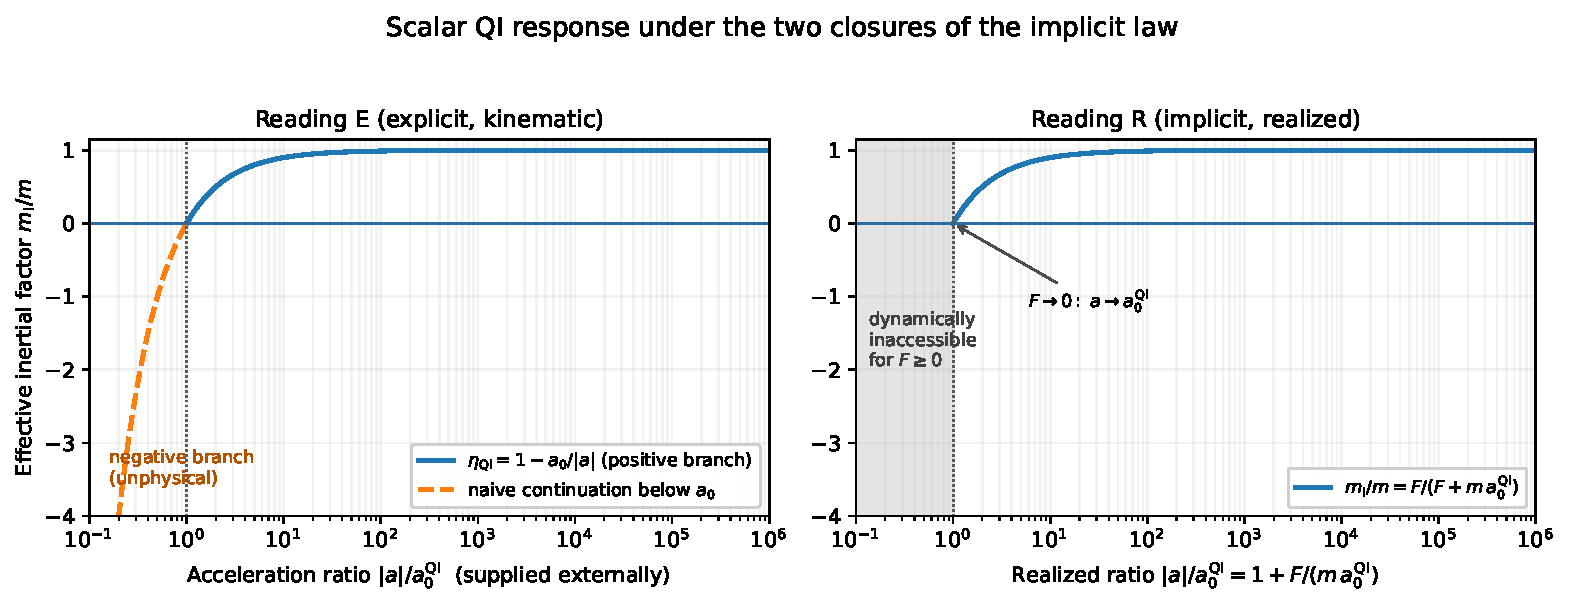
\includegraphics[width=0.82\textwidth]{qi_scalar_response.pdf}
    \caption{The scalar QI response \(m_{\mathrm I}/m=1-a_{0}^{\QI}/|a|\) under the \emph{explicit kinematic} reading, in which \(|a|\) is an externally supplied acceleration. On that reading \(m_{\mathrm I}\ge0\) requires \(|a|\ge a_{0}^{\QI}\) and continuation below the threshold produces a negative inertial coefficient. Under the \emph{implicit realized} reading of \cref{sec:implicit_closure} the region \(|a|<a_{0}^{\QI}\) is dynamically inaccessible for \(F\ge0\), the plotted negative branch is never reached, and \(m_{\mathrm I}/m=F/(F+ma_{0}^{\QI})\) is automatically confined to \([0,1)\). The figure therefore displays a reading-dependent artefact, not an unavoidable defect of the scalar law.}
    \label{fig:scalar_response}
\end{figure}


\subsection{Input or realized acceleration: the implicit closure of the scalar law}
\label{sec:implicit_closure}

\Cref{eq:qi_main} is not an explicit formula. The effective inertial mass depends on \(a\), and in any dynamical use \(a\) is itself determined by \(m_{\mathrm I}\) through the equation of motion. The law is therefore implicit, and it admits two inequivalent closures. This is a distinct fork from the covariance question of \cref{sec:acceleration_obstruction}, and it must be settled independently.

\paragraph{Reading E (explicit, kinematic).} The symbol \(|a|\) denotes an acceleration supplied from outside the law, for example the Newtonian value \(F/m\) or a measured kinematic acceleration. Then
\begin{equation}
    \frac{m_{\mathrm I}}{m}
    =1-\frac{a_{0}^{\QI}}{|a|}
    \qquad\text{evaluated at a prescribed }|a|,
    \label{eq:reading_E}
\end{equation}
and the negative region of \cref{fig:scalar_response} is reachable.

\paragraph{Reading R (implicit, realized).} The symbol \(|a|\) denotes the acceleration actually realized by the body, so that \(m_{\mathrm I}\) and \(a\) must be solved together. For a one-dimensional applied force \(F\ge0\),
\begin{equation}
    F=m_{\mathrm I}a
    =m\left(1-\frac{a_{0}^{\QI}}{a}\right)a
    =m\left(a-a_{0}^{\QI}\right),
    \label{eq:qi_implicit}
\end{equation}
whence
\begin{equation}
    \boxed{\;
    a=\frac{F}{m}+a_{0}^{\QI},
    \qquad
    \frac{m_{\mathrm I}}{m}
    =\frac{F}{F+m\,a_{0}^{\QI}}
    \in[0,1).
    \;}
    \label{eq:qi_realized}
\end{equation}

Three consequences follow immediately, and they change the correct statement of several standard objections.

\begin{enumerate}[leftmargin=1.55em]
    \item \textbf{Positivity is automatic.} \Cref{eq:qi_realized} is non-negative for every \(F\ge0\) and monotone increasing in \(F\). No admissibility predicate, saturation law, or branch-matching condition is required.
    \item \textbf{The minimum acceleration is derived, not asserted.} Taking \(F\to0\) in \cref{eq:qi_realized} gives \(a\to a_{0}^{\QI}\). The floor that QI publications describe is the \(F\to0\) limit of the closed dynamics, not a separate postulate. The value \(a=0\) is never attained, so the singularity of \cref{eq:qi_eta} at \(a=0\) is not encountered on this reading.
    \item \textbf{The law becomes an additive acceleration floor.} \Cref{eq:qi_realized} states that the body acquires an irreducible acceleration \(a_{0}^{\QI}\) in addition to its Newtonian response. With \(\Theta\approx\SI{8.8e26}{m}\),
    \begin{equation}
        a_{0}^{\QI}=\frac{2c^{2}}{\Theta}\approx\SI{2e-10}{m.s^{-2}},
        \label{eq:a0_numeric}
    \end{equation}
    which is many orders of magnitude above the differential-acceleration noise floors reached by precision free-fall and torsion-balance experiments.
\end{enumerate}

The third consequence is the reason Reading R strengthens rather than weakens the audit, but it must be stated carefully, because \cref{eq:qi_realized} is the \(a'=0\) case of a more general relation and the general case is what the sources use. If the acceleration in \cref{eq:qi_realized} were proper or laboratory-frame acceleration, an absolute floor at \SI{2e-10}{m.s^{-2}} would already be excluded by existing free-fall data. It is not, and \cref{sec:decomposition} shows exactly how the programme avoids that bound. The positivity question therefore does not open a second unresolved issue: it collapses into the acceleration-definition question of \cref{sec:acceleration_obstruction} and makes it more urgent, because what has to be specified turns out to be not merely a covariant scalar but a summation rule over surrounding matter.

\subsection{The acceleration-decomposition postulate}
\label{sec:decomposition}

\Cref{eq:qi_realized} applied to a circular orbit with \(F=GMm/r^{2}\) and \(a=v^{2}/r\) gives
\begin{equation}
    v^{2}=\frac{GM}{r}+a_{0}^{\QI}r,
    \label{eq:closure_R_rotation}
\end{equation}
so \(v\propto\sqrt{r}\) asymptotically. The relation reported for galaxy rotation under QI is instead the flat Tully--Fisher form
\begin{equation}
    v^{4}=GM\,a_{0}^{\QI}=\frac{2GMc^{2}}{\Theta}.
    \label{eq:closure_G_rotation}
\end{equation}
\Cref{eq:closure_R_rotation,eq:closure_G_rotation} are not the same relation, and the reason is instructive. It is not that the programme uses two different closures. It is that the published galactic derivation applies the closure to a \emph{decomposed} acceleration, and the decomposition rule carries the physical content.

The primary derivation writes the QI factor with \(|A|\), defined as the total of all accelerations of the star relative to nearby matter, and splits it into a mean rotational part \(a=v^{2}/r\) and a variable small-scale part \(a'\) \cite{McCulloch2012}:
\begin{equation}
    m\left(1-\frac{a_{0}^{\QI}}{|a|+|a'|}\right)a=\frac{GMm}{r^{2}}.
    \label{eq:mcculloch_decomposed}
\end{equation}
Multiplying through by \(|a|+|a'|\),
\begin{equation}
    \left(|a|+|a'|-a_{0}^{\QI}\right)a
    =\frac{GM\left(|a|+|a'|\right)}{r^{2}}.
    \label{eq:mcculloch_master}
\end{equation}
Both published relations are specializations of \cref{eq:mcculloch_master}.
\begin{enumerate}[leftmargin=1.55em]
    \item \(a'=0\). Then \cref{eq:mcculloch_master} reduces to \(a=GM/r^{2}+a_{0}^{\QI}\), which is exactly \cref{eq:qi_realized}, and yields \cref{eq:closure_R_rotation}. This is the acceleration floor invoked for Proxima Centauri and the Jupiter-mass binaries \cite{McCulloch2024Proxima,McCulloch2026JuMBO}.
    \item \(a'=a_{0}^{\QI}\) at the galaxy's edge. Then the second and third terms on the left of \cref{eq:mcculloch_master} cancel identically, leaving \(a^{2}=GM(|a|+|a'|)/r^{2}\); with \(a\ll a'\) this gives \(a^{2}=GM a_{0}^{\QI}/r^{2}\) and hence \cref{eq:closure_G_rotation}.
\end{enumerate}

So there is one closure, and \cref{crit:closure_declaration} is satisfied by the primary sources. What is not supplied is a derivation of the decomposition. The source states the second specialization as an assumption: the residual minimum acceleration is taken to be found in smaller-scale motions of the stars. That assumption, not the scalar law, is what produces the Tully--Fisher relation, because it is precisely what cancels the \(a_{0}^{\QI}\) term in \cref{eq:mcculloch_master}. Three consequences follow.

\paragraph{(a) The acceleration is a scalar sum of magnitudes over an unspecified matter set.} \(|A|=|a|+|a'|\) adds the magnitudes of physically distinct accelerations: one orbital, one an unresolved ensemble of local motions. It is not a vector sum, not a covariant scalar, and not determined by the target worldline alone. This compounds \cref{sec:acceleration_obstruction} rather than resolving it. The object \(a_{\mathrm{rel}}\) is not merely covariantly undefined; it is defined by a summation rule whose domain is never stated, so two analysts given the same galaxy and the same stellar population can obtain different \(|A|\) and different predictions. A complete formulation must declare which matter enters the sum, at what scale, with what weighting, and why magnitudes rather than vectors are added.

\paragraph{(b) The floor is carried by \(|A|\), not by \(F/m\), and is therefore shielded from laboratory bounds.} This corrects the naive reading of consequence~3 above. Because \(|A|\) includes accelerations relative to all nearby matter, any terrestrial apparatus sits enormously far above \(a_{0}^{\QI}\), and the resulting equivalence-principle violation is stated by the source to lie below torsion-balance sensitivity \cite{McCulloch2011Tajmar}. That is an internally consistent position. Its cost is that the programme's most distinctive prediction is protected from every existing laboratory bound by a summation rule with no independent specification. Declaring the domain of the sum is consequently not a technical tidiness issue; it is the precondition for the floor being an empirical claim at all.

\paragraph{(c) The decomposition generates a real and apparently untested prediction.} The source draws the correct inference and states it plainly: at a galaxy's outer edge, small-scale stellar accelerations must \emph{increase} as the rotational acceleration falls with radius, so as to hold the total at the floor \cite{McCulloch2012}. This is a claim about the run of internal velocity dispersion with galactocentric radius, and it is checkable against resolved kinematics. It is developed as \cref{sec:aprime_test}, and it is the sharpest galactic test the programme currently offers, because unlike the Tully--Fisher fit it is not shared with MOND.

\begin{principle}[Closure declaration]
An implicit constitutive law is not specified by its algebraic form alone. A complete statement of \cref{eq:qi_main} must declare whether \(|a|\) is an externally supplied kinematic input or the realized acceleration of the closed equation of motion, must use the same declaration in every application, and must derive rather than assume any acceleration floor that follows.
\label{prin:closure}
\end{principle}

\subsection{The proposed physical mechanism}

The QI mechanism combines two distinct restrictions. First, a uniformly accelerated observer has a Rindler wedge and associates the Minkowski vacuum with a thermal response at the Unruh temperature \cite{Fulling1973,Davies1975,Unruh1976,Crispino2008}. QI proposes that the associated horizon removes or suppresses modes on the side opposite acceleration, creating an anisotropic radiation pressure that resists acceleration \cite{McCulloch2013}. Second, at very low acceleration the relevant Unruh wavelengths become so large that a cosmic boundary is proposed to suppress them in all directions, reducing inertial response \cite{McCulloch2007,McCulloch2010}.

This is a mechanistic claim, not merely a modified equation of motion. It requires at least four bridges:
\begin{equation}
\begin{aligned}
\text{accelerated detector/observer response}
&\longrightarrow \text{mode asymmetry}\\
&\longrightarrow \text{renormalized stress imbalance}\\
&\longrightarrow \text{universal inertial reaction}.
\end{aligned}
\label{eq:mechanism_bridges}
\end{equation}
Each arrow has independent mathematical content. The Unruh result establishes neither a one-sided stress nor a universal force automatically, and universality across particles, composites, fields, neutral bodies, binding energies, and macroscopic carriers is a further burden.

\subsection{Which acceleration enters the law?}
\label{sec:acceleration_obstruction}

The acceleration entering the standard Unruh relation is proper acceleration. For a worldline with four-velocity \(u^{\mu}\),
\begin{equation}
    a_{\mathrm{prop}}^{\mu}:=u^{\nu}\nabla_{\nu}u^{\mu},
    \qquad
    a_{\mathrm{prop}}:=\sqrt{-a^{\mu}_{\mathrm{prop}}a^{\mathrm{prop}}_{\mu}}
\end{equation}
for the \((+---)\) convention. A geodesic satisfies
\begin{equation}
    a_{\mathrm{prop}}^{\mu}=0.
    \label{eq:geodesic_proper_acceleration}
\end{equation}
A star following a gravitational orbit is locally in free fall and therefore does not possess the proper acceleration required to generate the ordinary Rindler detector temperature from its orbital motion.

The QI source instead defines \(a\) as acceleration ``relative to surrounding matter'' \cite{McCulloch2016}. That may be intended as a relational or coordinate acceleration, but then the Rindler inference is no longer automatic. A covariant formulation would have to supply a physically preferred timelike congruence \(U^{\mu}\) representing the surrounding matter and a scalar functional
\begin{equation}
    a_{\mathrm{rel}}
    =\mathcal A[u,U,g,\nabla U,\ldots]
    \label{eq:relational_acceleration_placeholder}
\end{equation}
that is invariant under coordinate changes, fixed independently of the target orbit, and shown to generate the same detector response used in the horizon derivation.

The theory therefore faces a precise fork:
\begin{enumerate}[leftmargin=1.55em]
    \item If \(a=a_{\mathrm{prop}}\), the Rindler/Unruh step is covariant, but freely falling galactic stars have \(a=0\), so the published galactic mechanism is not obtained.
    \item If \(a=a_{\mathrm{rel}}\), low-acceleration orbital phenomenology may be defined, but a preferred congruence and a new bridge from \(a_{\mathrm{rel}}\) to Rindler thermality are required.
\end{enumerate}
Moreover, the scalar factor in \cref{eq:qi_eta} is undefined at \(a=0\); it does not reduce to unity there. A separate branch rule is therefore required even before the covariant acceleration question is closed. This acceleration-type ambiguity is more fundamental than a numerical coefficient mismatch because it determines whether the proposed horizon exists at all.


\subsection{The laboratory and galactic branches are not one tested law}
\label{sec:branch_nontransfer}

The acceleration fork has an immediate evidentiary consequence. In a field-emission capacitor, electrons experience a large nonzero proper acceleration, locally of order
\begin{equation}
    a_{\mathrm{prop}}\sim \frac{eE}{m_e}
\end{equation}
within the regime where a single-particle description is adequate. A star following a galactic geodesic instead satisfies \(a_{\mathrm{prop}}^{\mu}=0\). QI's laboratory branch can therefore be written schematically as
\begin{equation}
    \mathrm{QI}_{\mathrm{lab}}=\mathrm{QI}[a_{\mathrm{prop}},\rho,\Bdy,\text{carrier}],
\end{equation}
whereas the galactic branch requires
\begin{equation}
    \mathrm{QI}_{\mathrm{gal}}=\mathrm{QI}[a_{\mathrm{rel}},U^{\mu},\Theta,\text{orbit}].
\end{equation}
Until a covariant map from \(a_{\mathrm{rel}}\) to the detector/horizon response is derived, these are not two independent tests of one closed law. They are two model branches using inequivalent acceleration objects. Consequently,
\begin{equation}
    \text{support for }\mathrm{QI}_{\mathrm{lab}}
    \not\Rightarrow
    \text{support for }\mathrm{QI}_{\mathrm{gal}},
    \qquad
    \text{and conversely}.
    \label{eq:branch_nontransfer}
\end{equation}
A future unification must state the preferred congruence, transformation law, and common action or response functional before evidence can transfer across the two branches.

\subsection{The public Fortran implementation as an acceleration audit target}
\label{sec:fortran_audit}

A public author post dated 24 November 2025 reports a Fortran model intended to simulate ``complete QI dynamics.'' The description says that the trajectory is initialized from JPL Horizons data, that QI reduces inertial mass and centrifugal response in the low-acceleration outer Solar System, and that the model predicts a return of 3I/Atlas \cite{McCullochFortran2025}. The public description does not provide the update equations or source code. It therefore does not establish which acceleration enters the scalar correction.

The implementation supplies a potentially decisive audit target. Define
\begin{equation}
 a_{\mathrm{code}}
 \in
 \left\{
 a_{\mathrm{prop}},
 a_{\mathrm{coordinate}},
 a_{\mathrm{relative\ matter}},
 a_{\mathrm{hybrid}}
 \right\}.
 \label{eq:code_acceleration_classes}
\end{equation}
A reproducible code release should state the reference frame, the acceleration inserted into \cref{eq:qi_main}, its transformation under a change of frame, whether geodesic free fall gives \(a_{\mathrm{code}}=0\), and whether the same object enters the capacitor branch. If the code evolves heliocentric coordinate acceleration, the result is a preferred-frame or relational modified-inertia model rather than the proper-acceleration law used in the standard Unruh formula. That outcome would not make the numerical model meaningless, but it would empirically confirm the branch split in \cref{eq:branch_nontransfer}.

\subsection{Astrophysical and laboratory extensions}

QI has been applied to the Pioneer and flyby anomalies, minimum galaxy accelerations, galaxy rotation curves, dwarf systems, wide binaries, Proxima Centauri, and more recently the inferred mutual accelerations of Jupiter-mass binary objects \cite{McCulloch2007,McCulloch2010,McCulloch2012,McCulloch2017Galaxy,McCullochLucio2019,McCulloch2024Proxima,McCulloch2026JuMBO}. These applications do not all test the same statistical object. Some fit mean rotation speeds, some identify a lower envelope, some use one system, and some predict a distributional shift. Their evidentiary status must therefore be evaluated separately.

The laboratory branch proposes that conducting or dielectric boundaries can replace horizons as mode-restricting structures. The supplied capacitor model predicts
\begin{equation}
    F_{\QI}
    \simeq
    1.4\times10^{-4}\frac{IA}{d^{2}},
    \label{eq:capacitor_force}
\end{equation}
with force toward the anode, current \(I\), active plate area \(A\), and separation \(d\) \cite{McCulloch2021Capacitors}. The relation is scientifically useful because it is specific: linear in \(I\) and \(A\), inverse-square in \(d\), and nominally independent of voltage when current is held fixed. The same specificity also means that partial agreement with one data set cannot close the mechanism if plate thickness, material response, conductor placement, field-emission regime, and total momentum remain unmodelled.

\section{Framework-independent physical background}
\label{sec:background}

\subsection{Rindler thermality is not a stress-energy wind}

The Fulling--Davies--Unruh result concerns the representation of a quantum field with respect to accelerated time translations. A uniformly accelerated detector coupled to a field in the Minkowski vacuum responds thermally with temperature
\begin{equation}
    T_{\mathrm U}=\frac{\hbar a_{\mathrm{prop}}}{2\pi c k_{\mathrm B}}.
    \label{eq:unruh_temp}
\end{equation}
The Bisognano--Wichmann result identifies the Minkowski vacuum restricted to a Rindler wedge as a KMS state with respect to the boost generator \cite{BisognanoWichmann1975,Crispino2008}. This is a statement about modular/boost thermality and detector response, not the appearance of a new local material medium.

With the standard Minkowski-vacuum renormalization,
\begin{equation}
    \avg{0_{\mathrm M}|T_{\mu\nu}|0_{\mathrm M}}_{\mathrm{ren}}=0
    \label{eq:minkowski_stress_zero}
\end{equation}
throughout flat spacetime, including points inside the Rindler wedge. Restricting the state to the wedge changes the algebraic description and yields the KMS property, but it does not change the local expectation value into a one-sided radiation stress. Explicit Rindler-wedge stress-tensor calculations likewise recover zero relative stress at the Unruh temperature \cite{MorettiVanzo1996}. Therefore the baseline QI force candidate satisfies
\begin{equation}
    F^{(0_{\mathrm M})}_{i}
    =\int_{\partial V}
    \avg{0_{\mathrm M}|T_{ij}|0_{\mathrm M}}_{\mathrm{ren}}
    n^{j}\,\dd A
    =0.
    \label{eq:rindler_baseline_force_zero}
\end{equation}

The detector response does not reopen that ledger. Unruh and Wald showed that what the accelerated description calls absorption of a Rindler quantum corresponds, in the inertial description, to emission of a real Minkowski quantum; the required energy is supplied by the external agency maintaining the acceleration \cite{UnruhWald1984}. Ordinary field momentum and radiation reaction already close the complete system.

Consequently, a Rindler decomposition of the Minkowski vacuum alone cannot provide the proposed pressure imbalance. A nonzero force requires additional physical structure, such as a material boundary, a non-Minkowski state, nonuniform or finite-duration acceleration, switching, dissipation, detector backreaction, or a boundary-modified stress tensor. Those additions may be legitimate, but they must be specified and calculated rather than attributed to Unruh thermality itself.


\subsection{The Fulling-Rindler vacuum does not supply the required directed thrust}
\label{sec:fulling_vacuum}

A possible response to the Minkowski-vacuum result is to replace the field state by the Fulling--Rindler vacuum. That move changes the physical problem. Moretti and Vanzo use the \((-+++)\) convention; translated to the \((+---)\) convention used throughout this paper, their massless-scalar stress tensor at dimensionless inverse Rindler temperature \(\vartheta_{\mathrm R}\), relative to the Minkowski vacuum, is
\begin{equation}
    \Delta\avg{T^{ab}}_{\vartheta_{\mathrm R}}
    =\frac{1}{1440\pi^{2}\xi^{4}}
      \left[\left(\frac{2\pi}{\vartheta_{\mathrm R}}\right)^{4}-1\right]
      \left(4v^{a}v^{b}-g^{ab}\right),
    \qquad v^{a}v_{a}=1,
    \label{eq:rindler_thermal_stress}
\end{equation}
where \(\xi\) is the Rindler radial coordinate \cite{MorettiVanzo1996}. At \(\vartheta_{\mathrm R}=2\pi\), the state is the Minkowski vacuum and the relative stress vanishes. In the zero-temperature limit \(\vartheta_{\mathrm R}\to\infty\), corresponding to the Fulling vacuum, the comoving energy density is
\begin{equation}
    \rho_{\mathrm F}
    :=v_{a}v_{b}\Delta\avg{T^{ab}}_{\mathrm F}
    =-\frac{3}{1440\pi^{2}\xi^{4}}
    =-\frac{1}{480\pi^{2}\xi^{4}},
    \label{eq:fulling_negative_density}
\end{equation}
while the comoving momentum flux vanishes,
\begin{equation}
    q^{a}_{\mathrm F}
    :=-h^{a}{}_{c}\Delta\avg{T^{cd}}_{\mathrm F}v_{d}
    =0,
    \qquad
    h^{a}{}_{c}:=\delta^{a}{}_{c}-v^{a}v_{c}.
    \label{eq:fulling_zero_flux}
\end{equation}
The state therefore has a negative, horizon-divergent bulk stress but no directed radiation wind. Parentani's global analysis further shows that singular horizon contributions complicate the total-energy accounting rather than converting the state into a regular forward flux \cite{Parentani1993}.

The Fulling--Rindler vacuum is also not the state occupied simply because a material body accelerates through a field prepared in the Minkowski vacuum. It is a different, horizon-singular state defined by absence of Rindler quanta. Selecting it requires an independent state-preparation argument and does not rescue the original QI inference from Minkowski-vacuum Unruh thermality to mechanical pressure.

\subsection{Casimir boundaries and stress-energy}

The ideal parallel-plate Casimir force is
\begin{equation}
    F_{\mathrm C}=-\frac{\pi^{2}\hbar c}{240}\frac{A}{d^{4}},
    \label{eq:casimir}
\end{equation}
for perfectly conducting plates at zero temperature in the idealized geometry \cite{Casimir1948,BrownMaclay1969,Milton2001}. Its reliable derivations can be expressed through changes in vacuum energy, mode summation with regularization, scattering theory, or the renormalized expectation value of the stress tensor. The physical result depends on geometry, material response, temperature, finite conductivity, roughness, and boundary conditions. ``Mode removal'' is a useful shorthand, but the force is not obtained by deleting arbitrary wavelengths and multiplying the remainder by a pressure factor.

For a candidate boundary-induced force, the generic burden is
\begin{equation}
    F_i
    =\int_{\partial V}
    \Delta\avg{T_{ij}}_{\mathrm{ren}}n^{j}\,\dd A,
    \label{eq:stress_force}
\end{equation}
with a declared state, field content, material response, renormalization prescription, and system boundary. If matter exchanges momentum with a field, that field momentum must appear in the complete ledger.

\subsection{Inertial mass and complete-system mass}

For a complete relativistic system,
\begin{equation}
    P_{\mu}P^{\mu}=M^{2}c^{2}
    \label{eq:mass_casimir}
\end{equation}
using the \((+---)\) signature. The invariant mass \(M\) includes all contributions to the complete four-momentum: constituent masses, kinetic structure in the center-of-momentum frame, binding, fields, and stresses. Massless constituents can form a massive composite if the total momentum is not null. Explicitly,
\begin{equation}
    M^{2}c^{4}=E_{\mathrm{tot}}^{2}-c^{2}\abs{\mathbf P_{\mathrm{tot}}}^{2}.
    \label{eq:composite_mass}
\end{equation}
Thus confinement of null modes can generate a nonzero mass for the complete configuration. This standard result does not establish that an electron is literally a photon in a loop, but it identifies the rigorous core beneath that intuition.

\section{Forensic audit I: uncertainty, energy, and the QI derivation}
\label{sec:uncertainty_audit}

\subsection{Expectation value and variance are different functionals}

The 2016 QI derivation explicitly proposes that the conserved quantity is not mass--energy alone but mass--energy plus an ``energy uncertainty,'' and that a horizon-induced reduction of positional uncertainty makes the latter physically available \cite{McCulloch2016}. Standard quantum mechanics distinguishes
\begin{equation}
    E_{\psi}:=\avg{H}_{\psi}
\end{equation}
from
\begin{equation}
    \Delta H_{\psi}
    :=\sqrt{\avg{H^{2}}_{\psi}-\avg{H}_{\psi}^{2}}.
    \label{eq:energy_variance}
\end{equation}
The first is the state expectation of the Hamiltonian. The second is the dispersion of possible energy outcomes. They have the same dimensions but not the same physical role.

The postulate
\begin{equation}
    mc^{2}+\Delta H=\mathrm{constant}
    \label{eq:qi_energy_postulate}
\end{equation}
therefore does not follow from the uncertainty principle. To make \(\Delta H\) an extractable work reservoir, one must specify a Hamiltonian coupling, a state transformation, a work protocol, a conserved current, and the complete energy balance of system plus apparatus. Without that structure, the term ``energy uncertainty becomes real'' is an additional constitutive hypothesis.

\begin{principle}[No variance-to-work implication]
A nonzero Hamiltonian variance does not by itself constitute additional mechanical energy. A work claim requires an explicit dynamical protocol connecting state preparation, coupling, measurement, backreaction, and conserved charge.
\end{principle}

This correction does not deny the objectivity of energy expectations or conserved charges. It prevents a different state functional, the Hamiltonian variance, from being reified as an additional reservoir merely because it carries the same physical units.

\subsection{The jurisdiction of the spectral uncertainty estimate}

Starting from
\begin{equation}
    \Delta p\,\Delta x\gtrsim \frac{\hbar}{2},
\end{equation}
QI writes an order-of-magnitude relation
\begin{equation}
    \Delta E\,\Delta x\sim\hbar c.
    \label{eq:de_dx}
\end{equation}
This replacement uses \(E\sim pc\), which is exact for a massless free mode and an ultrarelativistic approximation for some massive states. It is not a universal canonical energy--position uncertainty relation. Energy is the generator conjugate to a declared temporal parameter, while position has no universal self-adjoint time analogue. Equation~\eqref{eq:de_dx} can be a dimensional or spectral estimate in a specified massless sector; it cannot be applied indiscriminately to Planck-mass constituents, composite bodies, and arbitrary acceleration states.

\subsection{The gravity calculation is circular at the constant-setting step}

The proposed gravity derivation sums pairwise uncertainty terms among Planck masses and obtains an inverse-square form. The coupling is then fixed by inserting the Planck mass, which already contains \(G\). The source paper acknowledges that this introduces circular reasoning \cite{McCulloch2016}. The calculation may therefore recover dimensional structure, but it does not derive Newton's constant from premises independent of Newtonian gravity.

The same restriction applies generally to vacuum-based gravity proposals: obtaining a residual force in one carrier does not establish universal gravitation, and a constant imported through the chosen cutoff cannot be counted as independently recovered \cite{Puthoff1989,Carlip1993,Cole2001}.

\subsection{The coefficient mismatch remains an open bridge}

The uncertainty route produces the intended QI factor multiplied by
\begin{equation}
    2\pi b_{\mathrm W}
    =1.26546\ldots,
    \qquad
    b_{\mathrm W}=0.201405\ldots,
    \label{eq:wien_factor}
\end{equation}
where \(b_{\mathrm W}\) is the dimensionless wavelength-form Wien coefficient defined by
\begin{equation}
    \lambda_{\mathrm{peak}}
    =b_{\mathrm W}\frac{hc}{k_{\mathrm B}T}.
\end{equation}
The source rounds this coefficient to \(0.2\) and attributes the resulting twenty-six-percent mismatch to a crude spherical treatment of the Rindler horizon \cite{McCulloch2016}. The mismatch is not automatically fatal to a heuristic derivation, but it cannot be removed by verbal attribution. A field-theoretic horizon calculation must produce the coefficient, specify the response spectrum, and show why the same coefficient applies across inequivalent carriers.

\subsection{Positivity is closure-dependent, and the residual burden is the acceleration floor}
\label{sec:positivity_revised}

Under Reading E of \cref{sec:implicit_closure}, the scalar factor in \cref{eq:qi_eta} requires
\begin{equation}
    |a|\ge a_{0}^{\QI}
\end{equation}
if \(m_{\mathrm I}\ge0\) is imposed, and a complete constitutive law would then have to supply an admissibility predicate, a nonlinear saturation law, a branch transition with matching conditions, or an instability argument.

Under Reading R none of that is needed. \Cref{eq:qi_realized} gives \(m_{\mathrm I}/m=F/(F+ma_{0}^{\QI})\), which is non-negative and bounded above by unity for every \(F\ge0\). Positivity is a theorem of the closed dynamics rather than an imposed condition, and the minimum acceleration is its \(F\to0\) limit. An audit that presents the negative branch as an unresolved defect of QI is therefore auditing Reading E while the published applications use Reading R.

The residual burden is different and considerably sharper. Under Reading R the theory predicts a universal additive acceleration floor,
\begin{equation}
    a-\frac{F}{m}=a_{0}^{\QI}\approx\SI{2e-10}{m.s^{-2}},
    \label{eq:floor_prediction}
\end{equation}
for every body, every composition, and every binding state. Three declarations are then compulsory.
\begin{enumerate}[leftmargin=1.55em]
    \item \textbf{The domain of the acceleration sum.} \Cref{eq:floor_prediction} is written for \(F/m\), but the sources apply the floor to \(|A|=|a|+|a'|\), the summed magnitude of all accelerations relative to nearby matter \cite{McCulloch2012}. That choice is what keeps the floor below laboratory sensitivity \cite{McCulloch2011Tajmar}, and it is unspecified: which matter enters the sum, over what scale, with what weighting, and why magnitudes are added rather than vectors. Until this is declared, \(|A|\) is not computable from a system's description and the floor is not a testable statement.
    \item \textbf{Whether the floor is directional.} \Cref{eq:qi_realized} was closed for a one-dimensional force, and \(|A|\) is built by adding magnitudes. A vector or tensor closure must specify the direction of the floor and its behaviour under superposition, which neither the scalar law nor the magnitude sum fixes.
    \item \textbf{The status of the decomposition assumption.} The Tully--Fisher result follows from setting \(a'=a_{0}^{\QI}\) at a galaxy's edge, which cancels the floor term in \cref{eq:mcculloch_master} (\cref{sec:decomposition}). This assignment is asserted, not derived. A complete theory must derive the equilibrium partition between \(a\) and \(a'\), or else present \cref{eq:closure_R_rotation,eq:closure_G_rotation} as separate reductions with separate evidentiary standing.
\end{enumerate}

The present QI formula supplies the threshold and, under Reading R, a closed positive branch. What it does not supply is a declaration of which reading is intended, a vector closure, or a demonstration that one closure covers the laboratory, Solar-system, and galactic domains simultaneously.

\section{Forensic audit II: confinement, particle masses, and the status of the null constant}
\label{sec:particle_mass}

\subsection{The ordinary and reduced Compton wavelengths}

The ordinary electron Compton wavelength is
\begin{equation}
    \lambda_{\mathrm C}=\frac{h}{m_{e}c},
\end{equation}
whereas the reduced Compton wavelength is
\begin{equation}
    \bar\lambda_{\mathrm C}=\frac{\hbar}{m_{e}c}.
\end{equation}
The QI particle-mass calculation inserts the ordinary value \(\lambda_{\mathrm C}\approx\SI{2.426e-12}{m}\) into
\begin{equation}
    m\stackrel{?}{=}\frac{\hbar}{c\lambda_{\mathrm C}}
\end{equation}
while reporting the electron mass \cite{McCulloch2016,Tiesinga2021}. Algebraically,
\begin{equation}
    \frac{\hbar}{c\lambda_{\mathrm C}}
    =\frac{\hbar}{c}\frac{m_{e}c}{h}
    =\frac{m_{e}}{2\pi}.
    \label{eq:compton_2pi}
\end{equation}
The displayed equation and numerical result are therefore inconsistent by \(2\pi\). Replacing \(\lambda_{\mathrm C}\) with \(\bar\lambda_{\mathrm C}\) gives
\begin{equation}
    \frac{\hbar}{c\bar\lambda_{\mathrm C}}=m_{e},
\end{equation}
which is exact because \(\bar\lambda_{\mathrm C}\) is defined using \(m_{e}\). It is an identity, not an independent prediction.

The same discipline applies to proton, nuclear, and Planck-scale estimates. Inserting a known confinement length into \(\hbar/(cL)\) can generate the correct order of magnitude because it is the natural relativistic quantum scale. Predictive closure requires an independently derived eigenvalue problem that fixes \(L\), the dimensionless spectral coefficient, and the complete representation content.

\subsection{What a trapped-photon model would still have to derive}

Even if a closed null mode produces the correct mass scale, an elementary electron theory must derive:
\begin{equation}
\left\{
\begin{array}{l}
\text{electric charge and gauge coupling},\\
\text{spin }1/2\text{ and the Pauli--Lubanski invariant},\\
\text{fermionic statistics and exclusion},\\
\text{magnetic moment and radiative corrections},\\
\text{chirality and electroweak representation},\\
\text{particle--antiparticle structure},\\
\text{observed pointlike scattering bounds}.
\end{array}
\right.
\end{equation}
A circular photon orbit does not supply these properties merely by matching \(mc^{2}\). The disciplined positive statement is narrower: closed or confined modes can produce a mass-like invariant for the complete configuration, and the derivation of the Standard Model representation remains open.

\subsection{Cosmic corrections to masses and redshift}

The supplied explanatory transcript proposes a mass law of the form
\begin{equation}
    m(\Theta)
    \sim \frac{\hbar}{c}
    \left(\frac{1}{L}-\frac{2}{\Theta}\right)
    \label{eq:cosmic_mass_correction}
\end{equation}
for a confinement scale \(L\) \cite{McCullochTranscript2026}. The fractional cosmic correction is
\begin{equation}
    \frac{\delta m}{m}\sim\frac{2L}{\Theta}.
\end{equation}
For particle scales \(L\sim10^{-13}\)--\(10^{-12}\,\si{m}\) and \(\Theta\sim10^{26}\,\si{m}\), the effect is of order \(10^{-39}\)--\(10^{-38}\). It is therefore far too small in the displayed form to replace ordinary cosmological redshift.

A varying-mass redshift claim must also identify the dimensionless observable. Atomic spectra depend on combinations involving \(\alpha\), mass ratios, \(\hbar\), and the reference apparatus. A common rescaling of every standard is not directly observable. No such dimensionless closure is supplied in the source claim.

\subsection{A cavity may change dispersion without changing the invariant null constant}

The 2026 blog material speculates that light behaves as a pressure wave in a quantum background, that a cavity may slow it, and that engineering the vacuum might alter the usual speed limit \cite{McCullochBlog2026}. Standard cavity and material physics already permits a modified dispersion relation
\begin{equation}
    \omega^{2}=c^{2}k^{2}+\Pi(\omega,\mathbf k;\Bdy),
    \label{eq:dispersion}
\end{equation}
with phase and group velocities
\begin{equation}
    v_{\mathrm p}=\frac{\omega}{k},
    \qquad
    v_{\mathrm g}=\frac{\partial\omega}{\partial k}.
\end{equation}
Neither need equal \(c\). This does not establish a change in the local invariant null structure. The standard symbol \(c\) is retained because the reviewed sources do not derive a new carrier-independent null constant.

A genuine change in \(c\) would require evidence for a carrier-independent null-cone deformation, not merely a cavity delay, resonance shift, phase velocity, group velocity, or material refractive index.

\section{Horizon and boundary taxonomy}
\label{sec:taxonomy}

QI employs several objects under a common language of mode restriction. They must remain physically and mathematically distinct.

\begin{table}[H]
\centering
\caption{Horizon and boundary objects relevant to QI. Similar response algebra does not imply physical identity.}
\label{tab:horizon_taxonomy}
\begin{tabularx}{\textwidth}{>{\raggedright\arraybackslash}p{0.22\textwidth}>{\raggedright\arraybackslash}p{0.34\textwidth}X}
\toprule
Object & Standard role & Possible QI role \\
\midrule
Event horizon & Global causal boundary in a spacetime geometry & Analogy for one-sided mode inaccessibility \\
Rindler horizon & Observer/trajectory-dependent wedge boundary associated with uniform proper acceleration & Directional accessibility restriction \\
Cosmological horizon or scale & Global causal or observational scale in a cosmological model & Long-wavelength mode restriction and minimum acceleration \\
Conducting plate & Material boundary condition for electromagnetic fields & Artificial mode deselection replacing a horizon \\
Dielectric or cavity wall & Frequency-, polarization-, and material-dependent response & Tunable spectral filter \\
\bottomrule
\end{tabularx}
\end{table}

The strongest defensible inference is not that a capacitor is a black hole or that a material boundary is a causal horizon. It is that inequivalent boundaries can alter admissible mode support. Whether one dynamical response law unifies those cases is an open physical bridge, not a synonymy.

\begin{principle}[Boundary-class non-identity]
If two systems admit similar mode-selection formulae, they may belong to one comparison class of boundary response. They are not thereby the same physical object, the same horizon, or the same state-preparation problem.
\end{principle}

\section{The force bridge: from accelerated response to inertia}
\label{sec:force_bridge}

\subsection{Baseline no-go, boundary modification, and reaction force}

A complete inertia derivation must distinguish three quantities:
\begin{align}
    \mathcal R_{D}[\rho,\gamma] &:= \text{detector response along trajectory }\gamma,\\
    \avg{T_{\mu\nu}}_{\rho,\Bdy} &:= \text{renormalized field stress in state }\rho,\\
    F^{\mathrm{obs}}_{i} &:= \text{mechanical force registered by the carrier/apparatus}.
\end{align}
The Unruh effect constrains the first under specified conditions. The Casimir effect constrains the second after boundaries alter the state or Green function. The third follows only after coupling, backreaction, and momentum exchange are specified.

For the unbounded Minkowski vacuum, \cref{eq:minkowski_stress_zero,eq:rindler_baseline_force_zero} give the baseline no-go result:
\begin{equation}
    \mathcal R_D\neq0
    \quad\not\Rightarrow\quad
    \Delta\avg{T_{ij}}_{\mathrm{ren}}\neq0
    \quad\not\Rightarrow\quad
    F_i^{\mathrm{obs}}\neq0.
    \label{eq:unruh_no_force_implication}
\end{equation}
A QI pressure mechanism therefore requires an explicitly modified state or boundary problem. The appropriate force object is
\begin{equation}
    F_i
    =\int_{\partial V}
    \left[
    \avg{T_{ij}}_{\rho,\Bdy,\mathrm{ren}}
    -\avg{T_{ij}}_{0_{\mathrm M},\mathrm{ren}}
    \right]n^{j}\,\dd A,
    \label{eq:boundary_modified_force}
\end{equation}
with the field state, material response, geometry, renormalization, and accelerating agent included in one momentum ledger.

QI effectively assumes a constitutive chain
\begin{equation}
    \mathcal R_{D}
    \longmapsto
    \Delta\avg{T_{ij}}_{\Bdy,\mathrm{ren}}
    \longmapsto
    -m_{\mathrm I}a_{i}.
    \label{eq:unruh_to_force}
\end{equation}
Its completion would require:
\begin{enumerate}[leftmargin=1.55em]
    \item a covariantly defined acceleration variable valid for the target carrier;
    \item a quantum state and finite boundary geometry;
    \item the carrier's composition- and frequency-dependent response tensor;
    \item a renormalized stress, influence functional, or open-system derivation;
    \item the reaction on the apparatus, emitted radiation, and accelerating agency;
    \item recovery of the universality and equivalence properties measured in high-acceleration regimes.
\end{enumerate}
Absent such additional structure, the Minkowski-vacuum calculation yields zero rather than an unresolved positive force.

\subsection{Universality is not optional}

An electromagnetic mechanism acts directly on charged degrees of freedom. Inertia is registered by neutral atoms, nuclei, composite bodies, radiation-filled cavities, binding energy, and fields. A universal inertial map must therefore commute with carrier decomposition. If \(\Carrier_{1}\to\Carrier_{2}\) is a justified transformation preserving the complete physical state, then the inferred inertial relation should satisfy a covariance condition schematically of the form
\begin{equation}
    \Phi_{\Carrier_{1}\to\Carrier_{2}}\circ\Mcal^{I}_{\Carrier_{1}}
    =\Mcal^{I}_{\Carrier_{2}}\circ\Phi_{\Carrier_{1}\to\Carrier_{2}},
    \label{eq:carrier_covariance}
\end{equation}
where \(\Phi_{\Carrier_{1}\to\Carrier_{2}}\) is the carrier-transfer map, within stated approximation errors. The symbol \(\Phi\) is used here rather than \(\eta\) to avoid collision with the scalar QI factor \(\eta_{\QI}=m_{\mathrm I}/m\). Without such a relation, a charged-particle vacuum model may remain a carrier-specific force hypothesis rather than a universal account of inertia.

This is the ordinary universality burden of an inertia theory: a force mechanism acting directly on one carrier cannot be promoted to universal inertia until it transfers across the full stress-energy content of equivalent systems.

\section{Capacitor thrust: exact claims and unresolved closure}
\label{sec:capacitor}

\subsection{The published scaling law}

The supplied capacitor manuscript starts from the ideal Casimir expression and replaces \(\hbar\) by an applied electrical energy--time scale,
\begin{equation}
    \hbar
    \longrightarrow
    E\tau
    =\frac{\mathcal P_{\mathrm{el}}d^{2}}{\bar v^{\,2}},
    \label{eq:hbar_substitution}
\end{equation}
where \(\mathcal P_{\mathrm{el}}\) is electrical power and \(\bar v\) is the assumed mean electron transit speed \cite{McCulloch2021Capacitors}. The source first obtains the final speed
\begin{equation}
    v_{\mathrm f}=\sqrt{\frac{2eV}{m_e}}
\end{equation}
and then sets
\begin{equation}
    \bar v=\frac{v_{\mathrm f}}{2},
    \qquad
    \bar v^{\,2}=\frac{eV}{2m_e}.
    \label{eq:mean_transit_speed}
\end{equation}
Using \(\mathcal P_{\mathrm{el}}=IV\) in \cref{eq:casimir,eq:hbar_substitution,eq:mean_transit_speed} gives
\begin{equation}
    F
    =\frac{\pi^{2}cm_e}{120e}\frac{IA}{d^{2}}
    =\alpha_{\mathrm{avg}}\frac{IA}{d^{2}},
    \qquad
    \alpha_{\mathrm{avg}}
    =1.4019\times10^{-4}\,\si{N.A^{-1}}.
    \label{eq:alpha_average}
\end{equation}
The published coefficient is therefore reconstructible from the stated half-final-speed convention. If the final speed \(v_{\mathrm f}\), rather than \(v_{\mathrm f}/2\), is inserted into the same residence-time ansatz, the result is
\begin{equation}
    \alpha_{\mathrm{final}}
    =\frac{\pi^{2}cm_e}{480e}
    =3.5048\times10^{-5}\,\si{N.A^{-1}},
    \label{eq:alpha_final}
\end{equation}
a factor of four smaller. The coefficient is therefore dimensional and convention-dependent. The derivation remains a dimensional ansatz: it is not obtained by quantizing a driven electron--field system with material boundaries, and it is not equivalent to evaluating \cref{eq:stress_force}.

The manuscript nonetheless supplies a valuable falsifiable surface:
\begin{equation}
    F\propto I,
    \qquad
    F\propto A,
    \qquad
    F\propto d^{-2},
    \qquad
    \left.\frac{\partial F}{\partial V}\right|_{I,A,d}\simeq0.
    \label{eq:capacitor_scaling}
\end{equation}
Figure~\ref{fig:capacitor_scaling} shows the strong inverse-square separation dependence for representative currents. The source text describes the increase as ``exponential,'' but its own formula is a power law.

\begin{figure}[H]
    \centering
    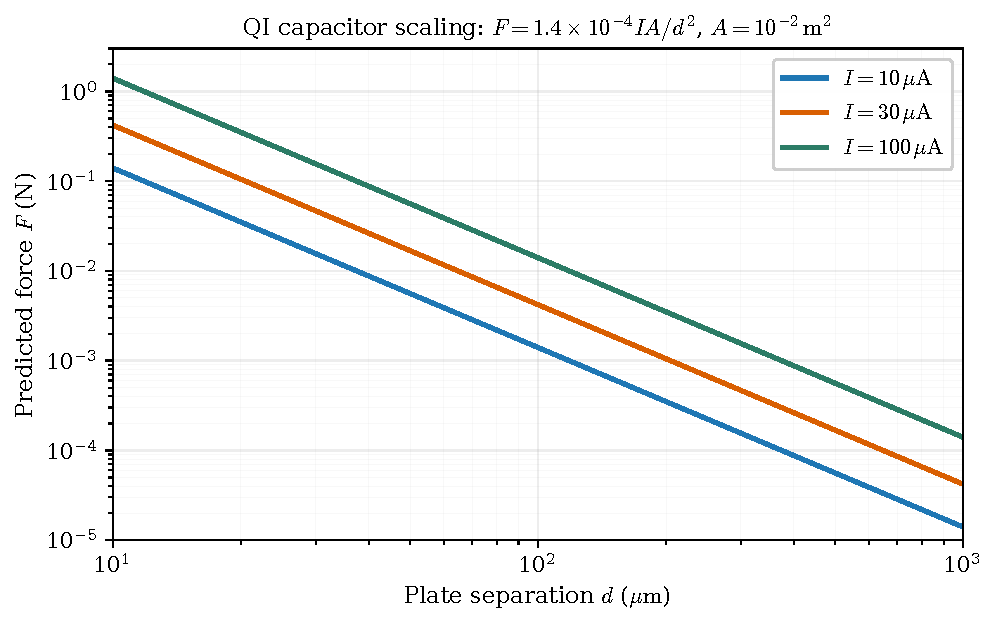
\includegraphics[width=0.82\textwidth]{qi_capacitor_scaling.pdf}
    \caption{Predicted capacitor force from \cref{eq:capacitor_force} for a fixed active area. The claim is an inverse-square power law in plate separation, not an exponential law. A valid test must vary current, area, separation, and voltage independently rather than collapse them into total power.}
    \label{fig:capacitor_scaling}
\end{figure}

\subsection{What the source acknowledges}

The capacitor paper states that it assumes complete blocking of the relevant Unruh modes by metal plates, that the damping factor is unknown, and that the model does not explain the observed effects of cathode thickness or all conductor placements \cite{McCulloch2021Capacitors}. These admissions are load-bearing. Plate thickness and nearby neutral conductors alter ordinary electrostatic fields, surface emission, charge transport, thermal paths, mechanical stress, and plasma formation. A QI interpretation must predict those dependencies before they are used as confirmation.

The claimed \(120\,\si{N\,kW^{-1}}\) performance is an extrapolation from preliminary field-emission measurements, not an established propulsion specification. The supplied 2026 blog recasts the capacitor as analogous to a small black hole and reproduces the same scaling, but the analogy adds no independent force derivation \cite{McCullochBlog2026}.

\subsection{Existing experiments and the correct comparison}

Bhatt and Becker reported bidirectional thrust-like signals in symmetric capacitors under field-emission conditions and conductor-placement changes \cite{BeckerBhatt2018}. Earlier asymmetric-capacitor work also shows that ion wind, leakage, outgassing, and electrohydrodynamic effects must be controlled with exceptional care \cite{Canning2004,MartinsPinheiro2011}.

Tajmar, K\"o{\ss}ling, and Neunzig performed high-vacuum, shielded, remotely controlled searches across capacitors, solenoids, material gradients, tunnelling-current devices, and crossed-field configurations, reporting no anomalous forces or torques down to nanonewton and nanonewton-metre sensitivity \cite{Tajmar2024}. Those tests strongly constrain broad steady-field gravity--electromagnetism couplings. They are not a one-to-one reproduction of the exact transient field-emission geometry used by Bhatt and Becker, so they do not alone close that specific claim. The correct conclusion is bounded:
\begin{equation}
\begin{split}
&\text{broad steady-field anomalous-force claims are strongly constrained;}\\
&\text{the exact transient QI capacitor scaling still requires a dedicated replication.}
\end{split}
\end{equation}

\subsection{Momentum closure}

``Propellantless'' cannot mean momentum from nothing. For a complete apparatus,
\begin{equation}
    \frac{\dd}{\dd\lambda}
    \left(
    P_{\mathrm{device}}+P_{\mathrm{field}}+P_{\mathrm{radiation}}
    +P_{\mathrm{boundary}}+P_{\mathrm{environment}}
    \right)=0
    \label{eq:momentum_ledger}
\end{equation}
in the complete physical description. The parameter \(\lambda\) indexes the experimental record. Any residual force must be accompanied by an identified momentum channel or by a new conservation law derived from a complete action.

\section{Astrophysical claims and their present status}
\label{sec:astro}

\subsection{Galaxy rotation}

QI has been applied to galaxy rotation curves using visible matter and the low-acceleration inertial reduction \cite{McCulloch2012,McCulloch2017Galaxy}. The programme's strength is parsimony: the acceleration scale is tied to a cosmic length rather than fitted separately for each galaxy. Its burden is correspondingly high. A valid comparison must include realistic baryonic mass uncertainties, distance and inclination errors, noncircular motions, stellar mass-to-light ratios, gas distributions, environment, and covariance across the full curve.

Agreement with a mean relation does not identify the QI mechanism because other frameworks can reproduce similar low-acceleration regularities. Differential evidence requires a prediction that competing models do not share, fixed before inspecting the target data.

\subsection{Wide binaries}

McCulloch and Lucio proposed that wide binaries provide a distributional test and predicted a characteristic high-velocity behaviour under QI \cite{McCullochLucio2019}. Renda independently identified major flaws in the original mode-counting derivation and obtained a different discrete spectrum \cite{Renda2019}. More importantly, a detailed Gaia DR3 distributional analysis by Banik and collaborators found the specific QI peak-shift prediction to be in catastrophic disagreement with the observed main peak and explicitly classified that QI proposal as falsified \cite{Banik2024}.

The surrounding gravity comparison, as distinct from the QI peak test, remains actively contested, and the exchange has continued past the point at which a single citation can summarize it. Pittordis, Sutherland, and Shepherd repeated the broader GR-versus-MOND comparison with more restrictive triple-contamination cuts, improved Gaia FLAME mass estimates, and refined mixture modelling; their Newtonian models fit significantly better than the tested MOND distributions, with the qualification that the unresolved-triple population must be understood more completely before the wider test is decisive \cite{Pittordis2025}. Cookson and collaborators then constructed a quality-controlled Gaia DR3 framework with aggressive astrometric, multiplicity, chance-alignment, and projection filtering, and reported that their cleanest sample shows no approximately twenty-percent MOND velocity enhancement \cite{Cookson2026}.

Both results have since been contested on sample-size and selection grounds. Chae and Yoon re-examined data quality control and multiple-star modelling in the projected-velocity tests and argue that the Cookson result rests on a small MOND-regime subsample together with inherited selection and mass-assignment choices; with a substantially larger sample under their own quality framework they recover a low-acceleration anomaly \cite{ChaeYoon2026}. Independently, Saad and Ting reanalysed the same thirty-six high-quality three-dimensional systems used by Chae and collaborators with a hierarchical Bayesian model that fits an explicit semi-major-axis parameter, and obtained a boost factor consistent with Newtonian gravity rather than the MOND-like value reported from the two-step consolidation \cite{SaadTing2026}. Other Gaia analyses continue to report low-acceleration anomalies or MOND-like enhancements \cite{Chae2023,ChaeEtAl2026}.

The correct summary is therefore symmetric rather than directional. The wide-binary gravity question is methodologically unsettled in both directions: the Newtonian-favouring analyses are disputed on sample construction, and the anomaly-favouring analyses are disputed on orbital modelling. None of this restores the specific QI distributional peak rejected by Banik and collaborators, because that rejection concerns a distinct predicted feature and not the size of a boost factor. The bounded conclusion stands: the tested QI prediction is rejected, the broader dispute is open, and neither later result constitutes a second direct QI test.

\subsection{Proxima Centauri}

A 2024 paper applies QI to Proxima Centauri and reports agreement with the observed orbital velocity within the observational bounds \cite{McCulloch2024Proxima}. The calculation is a one-system application with assumptions about binding, orbital state, mutual acceleration, and the absence of an external-field effect. A single-system agreement does not override a population-level distributional failure. The result remains a conditional fit requiring an orbit-level likelihood analysis under Newtonian, QI, and alternative models with the same data and priors.

\subsection{Jupiter-mass binary objects}

A 2026 paper reports that inferred mutual accelerations for 42 Jupiter-mass binary objects level near \(2c^{2}/\Theta\) and makes the sharper prediction that systems near a projected separation of approximately \(400\,\si{AU}\) should exhibit an orbital anomaly of about \(70\,\si{m.s^{-1}}\) \cite{McCulloch2026JuMBO,PearsonMcCaughrean2023}. This is currently one of the most useful QI claims because it points toward a prospective measurement. The existing inference depends on candidate status, projected separation, assumed masses, orbital orientation, cluster environment, and whether the objects are gravitationally bound. The proper test is therefore not retrospective visual alignment with a lower envelope. It is a preregistered radial-velocity and proper-motion distribution conditioned on the measured selection function.



\subsection{The residual-acceleration prediction}
\label{sec:aprime_test}

\Cref{sec:decomposition} identifies a prediction that is both sharp and, so far as the reviewed literature shows, untested. If the total relative acceleration cannot fall below \(a_{0}^{\QI}\), and if the mean rotational acceleration \(a=v^{2}/r\) falls with radius as it observably does, then the residual component must rise to compensate:
\begin{equation}
    |a'|(r)\;\ge\;a_{0}^{\QI}-\frac{v^{2}(r)}{r},
    \qquad\text{with equality at the equilibrium assumed in \cref{eq:closure_G_rotation}.}
    \label{eq:aprime_prediction}
\end{equation}
The source states the physical content directly: at a galaxy's outer edge, smaller-scale accelerations must increase to offset the decrease in rotational acceleration with radius \cite{McCulloch2012}.

This is the most valuable galactic prediction in the programme, for three reasons. It is not shared with MOND, which makes no claim about internal small-scale accelerations. It is differential rather than a mean-relation fit, so it escapes the objection of \cref{sec:astro} that agreement with a mean relation identifies no mechanism. And it concerns a quantity that resolved kinematics can measure.

A decisive test requires the prediction to be made operational, which the source does not do. Three declarations are needed before \cref{eq:aprime_prediction} can be confronted with data.
\begin{enumerate}[leftmargin=1.55em]
    \item \textbf{What \(a'\) physically is.} Candidate observables include the acceleration implied by the internal velocity dispersion \(\sigma\) over a coherence length \(\ell\), \(a'\sim\sigma^{2}/\ell\); accelerations from the local stellar and gas density field; or turbulent accelerations in the gas. These are not interchangeable and differ by orders of magnitude. One must be declared.
    \item \textbf{The scale over which the sum runs.} Since \(a'\) is an acceleration relative to nearby matter, its value depends on the radius within which neighbours are counted. A prediction that varies with an unstated aperture is not falsifiable.
    \item \textbf{The predicted radial profile.} \Cref{eq:aprime_prediction} must be converted into a curve \(\sigma(r)\) or equivalent, with error propagation, and compared against a preregistered Newtonian expectation.
\end{enumerate}

Given those declarations, the test is available now. Resolved stellar kinematics for nearby disc galaxies, together with gas velocity dispersion from radio surveys, already constrain the run of internal dispersion with radius. If dispersions do not rise in the outer disc in the manner \cref{eq:aprime_prediction} requires, the decomposition that generates the Tully--Fisher result fails, and \cref{eq:closure_G_rotation} loses its derivation while the scalar law itself remains untouched. That is precisely the branch-local failure structure this audit recommends throughout.

\subsection{Every astrophysical application lies at or below the threshold}
\label{sec:subthreshold}

The astrophysical claims of \cref{sec:astro} share a structural feature that is easy to miss when they are assessed one at a time. Each is evaluated in the regime where the QI correction is not a small perturbation but is of order unity or larger. Representative mutual accelerations are collected in \cref{tab:subthreshold}.

\begin{table}[H]
\centering
\caption{Newtonian mutual accelerations of the principal QI astrophysical targets compared with the QI threshold \(a_{0}^{\QI}=2c^{2}/\Theta\approx\SI{2e-10}{m.s^{-2}}\). Every target sits at or below the threshold.}
\label{tab:subthreshold}
\begin{tabularx}{\textwidth}{>{\raggedright\arraybackslash}p{0.24\textwidth}>{\raggedright\arraybackslash}p{0.26\textwidth}>{\raggedright\arraybackslash}p{0.18\textwidth}X}
\toprule
Target & Configuration & \(GM/r^{2}\) (\si{m.s^{-2}}) & \(GM/r^{2}\) relative to \(a_{0}^{\QI}\) \\
\midrule
Proxima Centauri & \(\sim2\,M_{\odot}\) at \(\sim\SI{13000}{AU}\) & \(\sim7\times10^{-11}\) & \(\sim0.35\) \\
JuMBO pair & two Jupiter masses at \SI{400}{AU} & \(\sim7\times10^{-11}\) & \(\sim0.35\) \\
Galaxy outskirts & flat-curve region & \(10^{-11}\)--\(10^{-10}\) & \(0.05\)--\(0.5\) \\
Wide binaries & \(2\)--\SI{30}{kAU} & \(10^{-11}\)--\(10^{-9}\) & \(0.05\)--\(5\) \\
\bottomrule
\end{tabularx}
\end{table}

Two audit consequences follow.

First, under Reading E of \cref{sec:implicit_closure} the displayed scalar law returns \(m_{\mathrm I}\le0\) for every entry in \cref{tab:subthreshold} except the high-acceleration end of the wide-binary range. The astrophysical programme therefore cannot be a test of \cref{eq:qi_main} as displayed under that reading. It is necessarily a test of the closure, and the closure is what \cref{sec:implicit_closure} shows is unstated.

Second, under Reading R the same entries are exactly the regime in which the realized acceleration is dominated by the floor rather than by the Newtonian term. In that regime \cref{eq:qi_realized} gives \(a\simeq a_{0}^{\QI}\) and \(m_{\mathrm I}\ll m\), so the predictions are governed almost entirely by the single cosmological constant \(a_{0}^{\QI}\) and almost not at all by the functional form of \cref{eq:qi_main}. Agreement in this regime consequently discriminates weakly between QI and any other theory carrying an acceleration scale near \(10^{-10}\,\si{m.s^{-2}}\).

The methodological corollary is that low-acceleration agreement is the least informative place to test QI, because it is where the theory has fewest free structural commitments. Differential power lies in the transition region \(|a|\sim a_{0}^{\QI}\), where Reading E and Reading R disagree sharply and where the functional form is actually exercised, and in the high-acceleration laboratory regime where the floor should be invisible and any residual force must come from the boundary mechanism instead. A revised QI programme should therefore preregister transition-region predictions rather than adding further deep-low-acceleration systems.

\subsection{Exploratory orbital commentary}

The supplied 2026 blog compilation includes an informal comparison between two satellites, one reportedly carrying a QI drive, while explicitly describing the reconstruction as subjective and acknowledging a possible Lorentz-force alternative \cite{McCullochBlog2026}. This is not an orbital demonstration. It is an anecdotal prompt for a controlled mission with matched spacecraft, telemetry, current profiles, magnetic characterization, attitude data, drag models, and predeclared orbit determination.

\section{Claim-status ledger}
\label{sec:ledger}

\begin{longtable}{>{\raggedright\arraybackslash}p{0.29\textwidth}>{\raggedright\arraybackslash}p{0.20\textwidth}>{\raggedright\arraybackslash}p{0.43\textwidth}}
\caption{Framework-independent claim-status ledger.}\label{tab:claim_ledger}\\
\toprule
Claim or object & Status & Correct interpretation \\
\midrule
\endfirsthead
\toprule
Claim or object & Status & Correct interpretation \\
\midrule
\endhead
Minkowski vacuum restricted to a wedge & Established KMS result & Thermal with respect to boosts; the local Minkowski-vacuum renormalized stress remains zero. \\
Rindler decomposition alone produces pressure & Rejected baseline mechanism & \(\langle T_{\mu\nu}\rangle_{0_M,\mathrm{ren}}=0\); additional state, boundary, switching, or material structure is required. \\
Fulling--Rindler vacuum supplies a regular outward wind & Rejected & In the \((+---)\) convention its comoving density is \(-1/(480\pi^2\xi^4)\) and its momentum flux vanishes. \\
Unruh detector excitation & Established result & Detector response is paid for by the accelerating agency; it is not a pre-existing one-sided wind. \\
QI acceleration variable & Covariantly unresolved & Proper acceleration supports the Unruh relation; galactic applications use an undefined relational acceleration. \\
Laboratory and galactic branches test one closed law & Not established & They use inequivalent acceleration objects until a covariant bridge is derived. \\
QI scalar law & Proposed map & Continuous low-acceleration reduction requiring an explicit closure declaration, a covariant acceleration, a vector form, and universality. \\
Negative inertial branch below \(a_{0}^{\QI}\) & Reading-dependent artefact & Present under the explicit kinematic reading; absent under the implicit realized closure \cref{eq:qi_realized}, where \(m_{\mathrm I}/m=F/(F+ma_{0}^{\QI})\in[0,1)\). \\
Minimum acceleration \(a_{0}^{\QI}\) & Derived under Reading R & The \(F\to0\) limit of the closed dynamics, not an appended admissibility rule. \\
Universal additive acceleration floor & Sharp but shielded consequence & \(a=F/m+a_{0}^{\QI}\) is the \(a'=0\) case; the sources apply the floor to \(|A|=|a|+|a'|\), which places every laboratory far above it and keeps the equivalence-principle violation below torsion-balance sensitivity. \\
One closure across all QI domains & Established from sources & Both published relations are specializations of \cref{eq:mcculloch_master}. The audit's earlier suspicion of two inequivalent closures is withdrawn. \\
Acceleration-decomposition rule \(|A|=|a|+|a'|\) & Undeclared and load-bearing & A scalar sum of magnitudes over an unspecified matter set; not covariant, not computable from a system description, and the source of the shielding above. \\
Assignment \(a'=a_{0}^{\QI}\) at a galaxy's edge & Asserted, not derived & It is what cancels the floor term and produces \(v^{4}=2GMc^{2}/\Theta\); no equilibrium argument fixes the partition between \(a\) and \(a'\). \\
Rising residual acceleration in the outer disc & Sharp untested prediction & Not shared with MOND and checkable against resolved kinematics; the strongest galactic test available (\cref{sec:aprime_test}). \\
Value of \(\Theta\) & Inconsistent across sources & \SI{2.7e26}{m} in the earlier papers versus \SI{8.8e26}{m} later, moving the floor by a factor of about \(3.3\) in a programme claiming no adjustable parameters. \\
Astrophysical targets sit at or below \(a_{0}^{\QI}\) & Audit inference & In that regime predictions are dominated by the single constant \(a_{0}^{\QI}\), so low-acceleration agreement discriminates weakly against any theory with a similar scale. \\
Hamiltonian variance is extra energy & Unsupported postulate & Same units do not imply the same physical account; a work protocol is absent. \\
Gravity from Planck-mass uncertainty & Incomplete derivation & Inverse-square form plus circular constant-setting through \(G\). \\
Electron mass from ordinary \(\lambda_C\) & Algebraically inconsistent & Gives \(m_e/(2\pi)\); the reduced wavelength returns \(m_e\) by definition. \\
Confined null modes can have mass & Established result & Complete-system invariant mass can be nonzero. \\
Electron is literally a trapped photon & Unsupported particle model & Charge, spin, statistics, chirality, couplings, and scattering structure remain un-derived. \\
Cavity changes group/phase velocity & Established possibility & Boundary-conditioned dispersion, not automatically variable fundamental \(c\). \\
Capacitor law \(F\propto IA/d^2\) & Sharp empirical hypothesis & Coefficient reconstructed only with the half-final-speed convention; exponents and voltage dependence require independent estimation. \\
\(120\,\si{N\,kW^{-1}}\) propulsion & Preliminary extrapolation & Requires independent replication and whole-system momentum closure. \\
Wide-binary QI peak prediction & Rejected tested map & Gaia DR3 distributional analysis rejects the specific prediction. \\
Later wide-binary comparison literature & Contested external results & Quality-controlled samples favour Newtonian fits; those analyses are in turn disputed on subsample size, selection, and orbital modelling. The dispute is open in both directions and contains no direct second QI test. \\
Public Fortran implementation & Open code-audit target & The public prose suggests coordinate or relational orbital acceleration; source code and update equations are required to classify the implemented acceleration and conservation law. \\
\bottomrule
\end{longtable}

\section{A decisive laboratory programme}
\label{sec:lab_programme}

\subsection{Experimental architecture}

The preferred apparatus is a battery-powered, optically read, high-vacuum system with no mechanical feedthrough during measurement. At minimum it should include:
\begin{enumerate}[leftmargin=1.55em]
    \item torsion and translational balances with independent calibration;
    \item electrostatic and magnetic shielding characterized over the switching spectrum;
    \item simultaneous current, voltage, field-emission, temperature, pressure, mass-loss, photon, X-ray, and vibration records;
    \item matched dummy loads reproducing power and heat without field emission;
    \item reversible apparatus orientation and electrode polarity;
    \item blind analysis and preregistered exclusions;
    \item raw data, code, calibration curves, and complete uncertainty propagation.
\end{enumerate}

\subsection{Factorial scaling test}

A proper test must vary \(I\), \(A\), \(d\), and \(V\) independently and estimate, rather than hard-code, the principal exponents. With reference values \(I_0,A_0,d_0,V_0,\mathcal P_0\), use the signed force model
\begin{align}
    F_{\mathrm{meas}}={}&
    F_0
    \left(\frac{I}{I_0}\right)^{p_I}
    \left(\frac{A}{A_0}\right)^{p_A}
    \left(\frac{d}{d_0}\right)^{-p_d}
    +\gamma_V(V-V_0)
    +\gamma_{\mathcal P}(\mathcal P_{\mathrm{el}}-\mathcal P_0)
    \notag\\
    &+\gamma_T\Delta T
    +\gamma_B B
    +\gamma_q\dot q
    +\varepsilon,
    \label{eq:factorial_model}
\end{align}
where the additive nuisance terms represent conventional couplings on the force scale. The QI capacitor prediction is
\begin{equation}
    p_I=1,
    \qquad
    p_A=1,
    \qquad
    p_d=2,
    \qquad
    F_0=\alpha_{\mathrm{avg}}\frac{I_0A_0}{d_0^2},
    \qquad
    \gamma_V\simeq0\ \text{at fixed }I.
    \label{eq:capacitor_exponent_predictions}
\end{equation}
The exponent test is now genuinely falsifiable. A log--log fit may be used for the positive QI component, but conventional thermal, magnetic, electrostatic, and leakage forces should remain additive unless a different physical model is justified.

\paragraph{Identifiability of the design.} \Cref{eq:factorial_model} is not automatically estimable, and a replication that ignores this will produce exponents with no meaning. Two obstructions must be handled explicitly.

The first is algebraic collinearity. Because \(\mathcal P_{\mathrm{el}}=IV\), the multiplicative term in \(I\), the additive term in \(V\), and the additive term in \(\mathcal P_{\mathrm{el}}\) are functionally related. They are formally distinct functions of \((I,V)\) and are therefore identifiable in principle, but the design matrix is near-singular for any operating envelope in which \(I\) and \(V\) move together. The protocol must accordingly report the condition number \(\kappa(\mathbf X)\) of the design matrix at the linearization point and satisfy a preregistered ceiling,
\begin{equation}
    \kappa(\mathbf X)\le\kappa_{\max},
    \label{eq:design_conditioning}
\end{equation}
with \(\kappa_{\max}\) fixed in advance and the variance-inflation factors for \(\gamma_V\) and \(\gamma_{\mathcal P}\) reported alongside the fitted exponents.

The second obstruction is physical and more serious. In a field-emission device the current is not an independent control variable: it is a Fowler--Nordheim function of the local field, so that
\begin{equation}
    I=I(V,d,\phi_{\mathrm{wf}},\beta_{\mathrm{fe}},A_{\mathrm{emit}}),
    \label{eq:fowler_nordheim_coupling}
\end{equation}
with \(\phi_{\mathrm{wf}}\) the work function, \(\beta_{\mathrm{fe}}\) the field-enhancement factor, and \(A_{\mathrm{emit}}\) the emitting area. Holding \(I\) fixed while sweeping \(V\) therefore requires changing \(d\), the emitter geometry, or the surface state, each of which moves another regressor in \cref{eq:factorial_model}. Taken literally, the QI prediction \(\gamma_V\simeq0\) at fixed \(I\) is close to untestable in a pure field-emission geometry, and any claimed confirmation of it in such a geometry should be treated as uninterpreted rather than as evidence.

The protocol must therefore include a decoupling stage. Acceptable options are an emitter with independently controllable gap and bias so that \((I,V,d)\) can be moved on a genuine three-factor grid; a thermionic or photoemission source in which the emission current is set by cathode temperature or illumination and is therefore controllable at fixed \(V\); or an externally injected beam current. Whichever is chosen, the preregistration must state the achieved factor ranges, the realized correlation matrix of \((\log I,\log A,\log d,V)\), and the resulting design conditioning. Without this, \cref{eq:capacitor_exponent_predictions} is a hypothesis that the apparatus cannot address.

\subsection{Boundary-reversal test}

The QI source set reports conductor-placement reversals relative to a proposed Rindler horizon \cite{BeckerBhatt2018,McCulloch2021Capacitors}. A decisive replication should pre-register the sign for each conductor position and include electrostatic finite-element modelling. Let \(s_{\Bdy}\in\{-1,0,+1\}\) encode the predicted sign. The result must satisfy
\begin{equation}
    \sgn(F_{\mathrm{res}})=s_{\Bdy}
\end{equation}
for held-out configurations. Post hoc placement-specific explanations do not count.

\subsection{Material-response test}

Perfect mode blocking is physically unrealistic. Introduce a measurable boundary response
\begin{equation}
    \mathscr D
    =\mathscr D
    (\omega,\mathbf k,\epsilon,\mu,\sigma_{\mathrm{cond}},t_{\mathrm{plate}},T,\Bdy).
    \label{eq:boundary_response}
\end{equation}
A completed QI map must predict how force changes with conductivity, thickness, surface state, dielectric loss, temperature, and frequency. If the force tracks ordinary charge leakage or surface emission rather than \(\mathscr D\) as predicted, the boundary-QI mechanism fails.

\subsection{Carrier-universality test}

If the mechanism is genuinely inertial rather than a special field-emission effect, appropriately normalized responses must transfer across independently characterized carriers. Candidate systems include electrons, neutral atoms, mechanical oscillators, field-filled cavities, and composite bodies. A result confined to field-emitting electrons would identify a carrier-specific electromagnetic or material phenomenon, not universal inertia. The test should freeze the response normalization, state preparation, and boundary model before comparing carriers; no cross-carrier support is earned by fitting an unrelated coefficient in each apparatus.

\subsection{Orientation and tensor test}

The proposed Rindler asymmetry is directional. The effective response should therefore be represented as
\begin{equation}
    F_i=\Mcal^{I}_{ij}a^{j},
\end{equation}
not assumed scalar in all geometries. Rotating the apparatus relative to acceleration, local gravity, the geomagnetic field, the laboratory, and the electrode normal can distinguish a boundary tensor from an uncontrolled environmental vector.

\subsection{Whole-system momentum test}

Force should be measured simultaneously on the device and on any emitted radiation or reaction products where possible. The test must quantify:
\begin{equation}
\left\{
\begin{array}{l}
\text{ion and neutral outflow},\\
\text{electron and photon momentum},\\
\text{electromagnetic interaction with shields and cables},\\
\text{thermal radiation and expansion},\\
\text{plasma pressure and ablation},\\
\text{support compliance and centre-of-mass motion}.
\end{array}
\right.
\end{equation}
A residual force that disappears when the complete momentum ledger is closed is not a QI signal.

\section{A decisive astrophysical programme}
\label{sec:astro_programme}

\subsection{Distributional rather than anecdotal tests}

Low-acceleration theories are often evaluated on selected systems or summary statistics. A stronger design predicts the full observable distribution. For wide binaries, this means a forward model for projected separation, relative velocity, unresolved companions, line-of-sight contamination, eccentricity, Galactic environment, and selection effects. The specific QI peak prediction already failed such a test \cite{Banik2024}. Any revised QI law must be frozen before application to a new release.

\subsection{JuMBO radial velocities}

For the Jupiter-mass binary claim, define a preregistered likelihood
\begin{equation}
    \mathcal L
    =\prod_{n=1}^{N}
    p\left(
    \Delta v_{r,n},\Delta\bm\mu_n,\rho_n
    \mid
    \mathcal M,\bm\theta,\mathcal S_{\mathrm{sel}}
    \right),
    \label{eq:jumbo_likelihood}
\end{equation}
where \(\mathcal M\) is Newtonian, QI, or an alternative dynamical model; \(\bm\theta\) contains masses and orbital parameters; and \(\mathcal S_{\mathrm{sel}}\) is the survey selection function. The key QI prediction should be stated in radial-velocity and proper-motion space, not only as an inferred acceleration floor from projected data.

\subsection{Redshift or cosmological dependence}

If \(\Theta\) is a genuine cosmological variable in the inertial law, the redshift dependence of \(a_{0}^{\QI}=2c^{2}/\Theta\) must be specified. Competing definitions---proper horizon, comoving diameter, Hubble radius, particle horizon, event horizon---are not interchangeable. A mature theory must declare which geometric object enters the law and how it transforms across cosmological epochs.

This is not a hypothetical concern. The value of \(\Theta\) used in the programme has itself changed. The earlier papers take \(\Theta=\SI{2.7e26}{m}\), described as the cosmic diameter at the epoch when the observed light was emitted, giving \(a_{0}^{\QI}=\SI{6.7e-10}{m.s^{-2}}\) \cite{McCulloch2012}; the later papers take \(\Theta=\SI{8.8e26}{m}\), the co-moving diameter at the present epoch, giving \(a_{0}^{\QI}\approx\SI{2e-10}{m.s^{-2}}\) \cite{McCulloch2017Galaxy,McCulloch2026JuMBO}. The predicted acceleration floor therefore differs by a factor of about \(3.3\) between publications of the same programme, with no adjustable parameter available to absorb the change. Since the floor is the quantity compared against Jupiter-mass binaries, Proxima, and galaxy edges, a declaration of which \(\Theta\) is intended, and a restatement of which published agreements survive under that choice, is a precondition for any cumulative empirical claim.

A smaller numerical point belongs here for completeness. The coefficient \(2\) in \(a_{0}^{\QI}=2c^{2}/\Theta\) is not exact: the source writes the correction as \(\beta\pi^{2}c^{2}/(|a|\Theta)\) with \(\beta\) the Wien coefficient rounded to \(0.2\) \cite{McCulloch2012}. With the exact wavelength-form value \(b_{\mathrm W}=0.201405\ldots\) of \cref{eq:wien_factor}, \(\pi^{2}b_{\mathrm W}=1.98779\ldots\), so the floor is \(\SI{0.6}{\percent}\) below the rounded value. This is negligible against the factor of \(3.3\) above, but a programme claiming to have no adjustable parameters should carry the unrounded constant.

\subsection{Composition and equivalence constraints}

QI changes inertial mass while ordinarily retaining gravitational mass. The proposal therefore implies a subtle effective violation of the strong equivalence between inertial and gravitational response in sufficiently low mutual-acceleration systems. The theory must state why high-precision terrestrial and Solar-system tests remain in the insensitive regime and whether composition, binding energy, or internal state changes the correction. ``Mass independence'' alone does not establish universality across all stress-energy sectors.

\section{Failure conditions and model selection}
\label{sec:failure}

The QI programme contains distinct physical branches. Each must have a finite failure domain, and evidence may not be transferred between branches without a derived bridge.

\begin{criterion}[Acceleration-definition failure]
The Rindler-based galactic mechanism fails if no covariant acceleration functional can both generate the required detector/horizon response and reproduce the orbital acceleration used in the scalar law without target-dependent preferred-frame choices.
\end{criterion}

\begin{criterion}[Closure-declaration failure]
\label{crit:closure_declaration}
The scalar law fails to be a determinate constitutive statement if it does not declare whether \(|a|\) is an externally supplied kinematic input or the realized acceleration of the closed equation of motion. Under the realized closure the theory additionally fails if the acceleration-decomposition rule \(|A|=|a|+|a'|\) is not given a stated summation domain, since without one \(|A|\) is not computable from a system's description and the acceleration floor is not an empirical claim; if the assignment \(a'=a_{0}^{\QI}\) that produces \cref{eq:closure_G_rotation} cannot be derived from an equilibrium argument rather than asserted; or if the residual-acceleration prediction of \cref{eq:aprime_prediction} is contradicted by resolved internal kinematics in the outer disc.
\end{criterion}

\begin{criterion}[Branch-unification failure]
The claim that laboratory and galactic QI constitute one theory fails if no common action, acceleration object, or response functional derives both \(\mathrm{QI}_{\mathrm{lab}}\) and \(\mathrm{QI}_{\mathrm{gal}}\). A confirmation in one branch then carries no evidentiary weight for the other.
\end{criterion}

\begin{criterion}[Implementation transparency failure]
A numerical QI result cannot test the covariant horizon mechanism unless the code identifies the acceleration object, reference frame, transformation rule, branch condition at zero acceleration, and conserved energy--momentum law. If the code uses a coordinate or preferred-frame acceleration, it tests that relational branch rather than the proper-acceleration Unruh mechanism.
\end{criterion}

\begin{criterion}[Laboratory QI failure]
The capacitor reduction fails if independent high-vacuum replications find no residual force at sensitivity well below \cref{eq:capacitor_force} across the preregistered scaling surface, or if observed forces track conventional variables while violating QI sign, voltage, material, or separation predictions.
\end{criterion}

\begin{criterion}[Force-bridge failure]
The Unruh-pressure mechanism fails as a universal inertia derivation if the baseline Minkowski-vacuum stress remains zero and no additional, independently specified boundary state yields a carrier-universal renormalized stress or influence-functional reaction proportional to inertial response.
\end{criterion}

\begin{criterion}[Particle-mass failure]
The trapped-mode programme fails as an elementary-particle theory if it cannot derive charge, spin, statistics, chirality, and coupling structure independently of the measured masses and Compton scales inserted into the calculation.
\end{criterion}

\begin{criterion}[Astrophysical QI failure]
A frozen QI reduction fails in a declared domain when its full predicted observable distribution is rejected after selection effects and nuisance populations are modelled. Retuning the horizon scale, acceleration definition, or environment rule after inspection constitutes a new model, not preservation of the original test.
\end{criterion}

\section{Discussion}
\label{sec:discussion}

\subsection{What QI gets structurally right}

QI directs attention to a serious possibility: inertial response may be relational, global, and boundary-sensitive. Its ratio \(\ellR/\LH\) expresses a local--global comparison rather than a purely intrinsic scalar. Its laboratory programme asks whether material boundaries can modulate a response ordinarily treated as fixed. Its astrophysical programme makes low-acceleration predictions rather than adding a separate invisible component to each target. These are substantive virtues of the research programme.

The strongest retained clue is boundary-conditioned spectral admissibility. Conducting, dielectric, geometric, and causal boundaries can alter the modes available to a physical carrier. That fact can change spectral energies, stresses, and complete-system mass without making Hamiltonian variance an additional energy substance.

\subsection{The two leading no-go results}

The first leading result is
\begin{equation}
    \text{Rindler KMS thermality of the Minkowski vacuum}
    \not\Rightarrow
    \text{nonzero local stress or directed pressure}.
\end{equation}
The baseline stress is zero. Choosing the Fulling-Rindler vacuum instead introduces a distinct, horizon-singular state with static negative bulk stress and no forward flux. Detector excitation is balanced by the accelerating agency. A QI force therefore requires a separately specified boundary or nonequilibrium state and a complete reaction calculation.

The second leading result is
\begin{equation}
    a_{\mathrm{prop}}\neq a_{\mathrm{rel}}
\end{equation}
in general. The former supports the standard Unruh/Rindler construction; the latter is used in galactic phenomenology but remains covariantly undefined. The capacitor and galaxy programmes cannot presently be counted as two lines of evidence for one law.

The third result is a correction to a common reading of the scalar law rather than an obstruction to it, and it is stated here because a fair audit must retract as well as add. \Cref{eq:qi_main} is implicit, and closing it on the realized acceleration gives \(a=F/m+a_{0}^{\QI}\) with \(m_{\mathrm I}/m=F/(F+ma_{0}^{\QI})\in[0,1)\). Positivity is then automatic and the minimum acceleration is derived. The frequently repeated objection that QI requires an ad hoc rule to avoid negative inertial mass applies only to the explicit kinematic reading, and this paper does not press it. What replaces that objection is stronger and more specific. Reconstructing the primary galactic derivation shows that the closure is applied to a decomposed acceleration \(|A|=|a|+|a'|\), and that both the JuMBO floor relation and the Tully--Fisher relation are specializations of one master equation. An earlier draft of this audit suspected two inequivalent closures; that suspicion is withdrawn. The genuine finding is that the physical work is done by the decomposition rather than by the scalar law: the summation domain of \(|A|\) is never declared, which simultaneously makes the floor non-computable from a system description and shields it from every laboratory bound, and the Tully--Fisher result follows from an asserted rather than derived assignment \(a'=a_{0}^{\QI}\). The positivity question therefore does not stand alongside the acceleration question; it reduces to it and sharpens it into a demand for a summation rule.

The remaining corrections are independently load-bearing: \(\avg{H}\neq\Delta H\), the gravity calculation imports \(G\), the ordinary Compton calculation misses by \(2\pi\), the reduced wavelength returns the mass by definition, and the capacitor derivation replaces \(\hbar\) by an applied action scale without deriving a boundary quantum state.

\subsection{Constructive frontier}

A completed QI theory would need:
\begin{enumerate}[leftmargin=1.55em]
  \item one covariant acceleration definition or an explicit declaration that laboratory and galactic branches are different theories;
  \item a declared quantum state and boundary algebra;
  \item a renormalized stress tensor or influence functional that produces a nonzero reaction from specified additional structure;
  \item complete momentum closure including the accelerating agency;
  \item universality across charged, neutral, composite, bound, and field carriers;
  \item one declared closure of the implicit scalar law, used consistently across the laboratory, Solar-system, and galactic domains, with a vector or tensor form and a conserved action;
  \item preregistered laboratory and astrophysical distributions.
\end{enumerate}
A derivation satisfying these conditions would move QI from a suggestive scalar programme toward a physically closed modified-inertia theory.

\section{Conclusion}
\label{sec:conclusion}

\begin{tcolorbox}[title=Final classification,colback=white,colframe=black]
Quantized inertia is a concrete and falsifiable but presently incomplete modified-inertia programme. Its boundary-spectral intuition remains scientifically valuable; its current Unruh-pressure, acceleration-unification, particle-mass, and capacitor-force bridges are not closed.
\end{tcolorbox}

The framework-independent audit yields firm results. The Minkowski vacuum restricted to a Rindler wedge is KMS with respect to boosts, but its local renormalized stress tensor remains zero. The Fulling-Rindler vacuum is a distinct, singular state and does not provide a directed forward momentum flux. The Unruh relation uses proper acceleration, whereas QI's galactic applications invoke acceleration relative to surrounding matter; without a covariant bridge, the laboratory and galactic programmes are not tests of one closed law. The scalar law is additionally implicit in \(a\): under the realized closure it becomes \(a=F/m+a_{0}^{\QI}\), positivity and the minimum acceleration follow as theorems rather than postulates, and the negative branch is a reading-dependent artefact rather than a defect. The cost of that closure is an acceleration floor near \SI{2e-10}{m.s^{-2}}, which the sources carry not on \(F/m\) but on a summed relative acceleration \(|A|=|a|+|a'|\) whose domain is never specified; that choice keeps the floor below laboratory sensitivity and simultaneously makes it non-computable from a system's description. Both published astrophysical relations follow from this one closure, so the audit's earlier suspicion of two inequivalent closures is withdrawn; the load is instead carried by an asserted assignment \(a'=a_{0}^{\QI}\) at a galaxy's edge, whose own consequence is that internal small-scale accelerations must rise in the outer disc. That consequence is not shared with MOND and is the sharpest galactic test presently available. Every astrophysical target of the programme lies at or below that threshold, where predictions are dominated by the single constant \(a_{0}^{\QI}\) rather than by the functional form under test. Hamiltonian variance is not automatically extractable energy. The relation \(\Delta E\,\Delta x\sim\hbar c\) has limited spectral jurisdiction. The gravity derivation imports \(G\) through the Planck mass. The inertia derivation retains the explicit factor \(2\pi b_{\mathrm W}=1.26546\ldots\). The ordinary-Compton-wavelength calculation gives \(m/(2\pi)\), while the reduced wavelength returns the mass by definition. Confined massless modes can form a massive composite, but an elementary electron theory must still derive its complete representation. A cavity can modify dispersion without changing the invariant null constant. The capacitor coefficient is reconstructible only after the source's half-final-speed residence convention is imposed; the force remains a precise but non-field-theoretic scaling hypothesis whose exponents must be estimated rather than assumed. The specific QI wide-binary distribution prediction is rejected; the broader wide-binary comparison remains unsettled in both directions, with quality-controlled Newtonian-favouring samples and their rebuttals on subsample size and orbital modelling both post-dating that rejection, while Proxima and the \(70\,\si{m.s^{-1}}\) JuMBO prediction remain conditional or prospective.

The decisive advance is methodological and physical. QI becomes most valuable when its horizon language is translated into a declared closure of the scalar law, a covariant acceleration, a nonzero boundary-modified stress tensor, complete momentum closure, and cross-carrier predictions that cannot be retuned after the fact. Its sharpest available test is not another deep-low-acceleration system but the transition region \(|a|\sim a_{0}^{\QI}\), where the competing closures make different predictions and the functional form is genuinely exercised. Until those bridges are supplied, QI should be evaluated branch by branch rather than treated as one already unified explanation of laboratory thrust, galactic dynamics, and elementary-particle mass.

\appendix

\section{Dimensional and algebraic audit}
\label{app:algebra}

\subsection{QI scalar law}

The correction term is dimensionless:
\begin{equation}
    \left[\frac{2c^{2}}{|a|\Theta}\right]
    =\frac{\si{m^2.s^{-2}}}{\si{m.s^{-2}}\,\si{m}}=1.
\end{equation}
The threshold acceleration \(2c^{2}/\Theta\) has the correct dimensions. Dimensional consistency does not determine the physical mechanism or the sign branch.

\subsection{Implicit closure of the scalar law}
\label{app:implicit_closure}

For one-dimensional applied force \(F\ge0\) and realized acceleration \(a>0\), substituting \cref{eq:qi_main} into \(F=m_{\mathrm I}a\) gives
\begin{equation}
    F=m\left(1-\frac{a_{0}^{\QI}}{a}\right)a
     =ma-ma_{0}^{\QI},
\end{equation}
which is linear in \(a\) with unit coefficient \(m\). Hence
\begin{equation}
    a=\frac{F}{m}+a_{0}^{\QI},
\end{equation}
and back-substitution gives
\begin{equation}
    \frac{m_{\mathrm I}}{m}
    =1-\frac{a_{0}^{\QI}}{\frac{F}{m}+a_{0}^{\QI}}
    =\frac{F/m}{\frac{F}{m}+a_{0}^{\QI}}
    =\frac{F}{F+ma_{0}^{\QI}}.
\end{equation}
The right-hand side is non-negative for all \(F\ge0\), equals zero only at \(F=0\), is strictly increasing in \(F\), and tends to unity as \(F\to\infty\). Therefore \(m_{\mathrm I}\in[0,m)\) and \(a\ge a_{0}^{\QI}\) identically, with equality only in the free limit. No admissibility predicate is required.

Two limits fix the interpretation. For \(F\gg ma_{0}^{\QI}\), \(a\to F/m\) and \(m_{\mathrm I}\to m\), recovering Newtonian dynamics. For \(F\to0\), \(a\to a_{0}^{\QI}\), which is the minimum acceleration reported in the QI literature. Note that the linearity of \cref{eq:qi_main} in \(a\) after multiplication is what makes the closure exactly solvable; a nonlinear interpolating factor would not admit this closed form and would generally reintroduce a branch question.

\subsection{Numerical value of the threshold}

With \(\Theta\approx\SI{8.8e26}{m}\),
\begin{equation}
    a_{0}^{\QI}
    =\frac{2c^{2}}{\Theta}
    =\frac{2\times(2.998\times10^{8})^{2}}{8.8\times10^{26}}
    \approx\SI{2.0e-10}{m.s^{-2}},
\end{equation}
which is the same order as the MOND acceleration scale and roughly four orders of magnitude above the differential-acceleration sensitivity of current precision free-fall instruments. The comparison in \cref{tab:subthreshold} uses this value throughout.

\subsection{Capacitor law}

For
\begin{equation}
    F=\alpha\frac{IA}{d^{2}},
\end{equation}
\(I\) is current, \(A\) is area, and \(d\) is length. Therefore \(IA/d^{2}\) has units of current, and \(\alpha\) is not dimensionless. Under the source's mean-transit-speed convention,
\begin{equation}
    \alpha_{\mathrm{avg}}
    =\frac{\pi^{2}cm_e}{120e}
    =1.4019\times10^{-4}\,\si{N.A^{-1}},
\end{equation}
whereas insertion of the final speed gives
\begin{equation}
    \alpha_{\mathrm{final}}
    =\frac{\pi^{2}cm_e}{480e}
    =3.5048\times10^{-5}\,\si{N.A^{-1}}.
\end{equation}
The coefficient therefore has the required units but depends on the residence-time convention. It should not be described as a pure parameter-free number.

\subsection{Ordinary Compton calculation}

Using
\begin{equation}
    \lambda_{\mathrm C}=\frac{h}{mc}=\frac{2\pi\hbar}{mc}
\end{equation}
produces
\begin{equation}
    \frac{\hbar}{c\lambda_{\mathrm C}}
    =\frac{\hbar}{c}\frac{mc}{2\pi\hbar}
    =\frac{m}{2\pi}.
\end{equation}
Using
\begin{equation}
    \bar\lambda_{\mathrm C}=\frac{\hbar}{mc}
\end{equation}
produces \(m\) identically. Any predictive use must derive the confinement length without importing the measured mass.

\section{Preregistered capacitor protocol template}
\label{app:protocol}

\begin{longtable}{>{\raggedright\arraybackslash}p{0.22\textwidth}>{\raggedright\arraybackslash}p{0.70\textwidth}}
\caption{Preregistration template for a decisive capacitor replication. Every row must be fixed and archived before force extraction.}\label{tab:capacitor_protocol}\\
\toprule
Protocol item & Required declaration \\
\midrule
\endfirsthead
\toprule
Protocol item & Required declaration \\
\midrule
\endhead
Primary hypothesis & Numerical coefficient, direction, current exponent, area exponent, separation exponent, and voltage dependence. \\
Primary outcome & Force or torque estimator, averaging window, filtering, calibration, and exclusion rule. \\
Geometry & Electrode dimensions, gap, thickness, surface treatment, alignment, support, shield, and conductor positions. \\
Electrical state & Current, voltage, pulse shape, duty cycle, field-emission onset, leakage, stored charge, and discharge path. \\
Factor decoupling & Mechanism by which \(I\) is varied independently of \(V\) (independent gap and bias control, thermionic or photoemission source, or injected beam), the achieved factor ranges, the realized correlation matrix of \((\log I,\log A,\log d,V)\), and the design condition number \(\kappa(\mathbf X)\) against its preregistered ceiling. \\
Environment & Pressure, gas composition, temperature, humidity, magnetic field, vibration, acoustic background, and radiation. \\
Controls & Dummy heater, non-emitting capacitor, reversed polarity, reversed orientation, shield configuration, and matched mass. \\
Blinding & Configuration code concealed from analysts until force extraction and quality cuts are frozen. \\
Momentum ledger & Ion, neutral, electron, photon, electromagnetic, thermal, and mechanical channels. \\
Failure condition & Sensitivity target below the QI force, with explicit rule for rejecting the scaling law. \\
Replication & Independent apparatus and team; raw data and code publicly archived. \\
\bottomrule
\end{longtable}

\section{Astrophysical test matrix}
\label{app:astro_matrix}

\begin{table}[H]
\centering
\caption{Minimum requirements for differential QI tests.}
\label{tab:astro_matrix}
\begin{tabularx}{\textwidth}{>{\raggedright\arraybackslash}p{0.18\textwidth}>{\raggedright\arraybackslash}p{0.24\textwidth}>{\raggedright\arraybackslash}p{0.27\textwidth}>{\raggedright\arraybackslash}X}
\toprule
Domain & QI object & Main nuisance structure & Decisive output \\
\midrule
Galaxy rotation & Full rotation-curve distribution & Distance, inclination, baryonic profile, noncircular motions & Held-out residual distribution versus common competitors \\
Wide binaries & Relative-velocity peak and tail & Close companions, projection, eccentricity, selection & Frozen forward-model likelihood; exact QI peak rejected, later quality-controlled analyses favour Newtonian over tested MOND distributions \\
Proxima & One wide triple orbit & Orbital phase, binding probability, central binary, priors & Common orbit likelihood under Newtonian and QI models \\
JuMBOs & Minimum mutual acceleration & Candidate status, mass, projection, cluster encounters & Test the predicted \(70\,\si{m.s^{-1}}\) anomaly near \(400\,\si{AU}\) in a full velocity distribution \\
Cosmology & Evolution of \(a_0^{\QI}\) & Definition of \(\Theta\), expansion model, selection & Redshift-dependent prediction fixed from one horizon definition \\
\bottomrule
\end{tabularx}
\end{table}

\section{Notation dictionary}
\label{app:notation}
\begin{tabularx}{\textwidth}{>{\raggedright\arraybackslash}p{0.21\textwidth}X}
\toprule
Symbol & Meaning \\
\midrule
\(m\) & Standard mass parameter or invariant mass in the relevant reduction. \\
\(m_{\mathrm I}\) & QI effective inertial mass. \\
\(a_{0}^{\QI}\) & QI minimum-acceleration scale \(2c^{2}/\Theta\approx\SI{2e-10}{m.s^{-2}}\). \\
\(\Theta\) & Cosmic diameter entering the QI law; taken as \(\approx\SI{8.8e26}{m}\) for numerical estimates. Its precise geometric definition---proper horizon, comoving diameter, Hubble radius, particle horizon, or event horizon---is not fixed by the reviewed sources. \\
\(\eta_{\QI}\) & Scalar QI factor \(m_{\mathrm I}/m=1-a_{0}^{\QI}/|a|\). Distinct from the carrier-transfer map \(\Phi_{\Carrier_1\to\Carrier_2}\). \\
Reading E, Reading R & Explicit kinematic and implicit realized closures of the scalar law; see \cref{sec:implicit_closure}. \\
\(\Phi_{\Carrier_1\to\Carrier_2}\) & Carrier-transfer map in the universality condition \cref{eq:carrier_covariance}. \\
\(\Mcal^{I}_{ij}\) & Tensorial inertial-response object replacing the scalar factor in general geometries. \\
\(\kappa(\mathbf X)\) & Condition number of the capacitor factorial design matrix. \\
\(a^{\mu}_{\mathrm{prop}}\) & Proper four-acceleration entering the standard Unruh relation. \\
\(a_{\mathrm{rel}}\) & As-yet undefined covariant relational acceleration required by QI orbital applications. \\
\(|A|,a,a'\) & Total summed relative acceleration in the source's galactic derivation, its mean rotational part \(v^{2}/r\), and its residual small-scale part. The summation domain of \(|A|\) is not specified by the reviewed sources. \\
\(\ellR\) & Rindler accessibility length \(c^{2}/|a|\). \\
\(\LH\) & Cosmic half-diameter \(\Theta/2\). \\
\(\Bdy\) & Boundary configuration and constitutive data. \\
\(\mathcal R_D\) & Detector response functional. \\
\(\avg{T_{\mu\nu}}_{\rho,\Bdy}\) & Renormalized field stress in state \(\rho\) and boundary configuration \(\Bdy\). \\
\(\vartheta_{\mathrm R}\) & Dimensionless inverse Rindler temperature; the Minkowski state occurs at \(\vartheta_{\mathrm R}=2\pi\). \\
\(b_{\mathrm W}\) & Wien wavelength coefficient \(0.201405\ldots\), so \(2\pi b_{\mathrm W}=1.26546\ldots\). \\
\(\mathcal P_{\mathrm{el}}\) & Electrical power, distinguished from four-momentum \(P^{\mu}\). \\
\(v_{\mathrm f},\bar v\) & Final and assumed mean electron transit speeds in the capacitor ansatz. \\
\(a_{\mathrm{code}}\) & Acceleration variable actually implemented in a numerical QI model. \\

\bottomrule
\end{tabularx}

\section*{Declarations}
\paragraph{Author contributions.}
Conceptualization, source assessment, formal analysis, methodology, investigation, and writing: H.A.-P. The author assumes responsibility for the final manuscript.

\paragraph{Funding.}
No external funding was received for this study.

\paragraph{Competing interests.}
The author declares no competing interest relevant to the framework-independent analysis.

\paragraph{Data and code availability.}
No new experimental dataset was generated. The scalar-response and capacitor-scaling figures are generated from the equations displayed in the manuscript; the plotting script, source figures, LaTeX file, and bibliography are included in the accompanying Overleaf package. Data and code for cited external studies remain subject to their respective source statements.

\paragraph{Use of computational tools.}
Computational tools supported source organization, algebraic verification, figure generation, bibliography preparation, LaTeX compilation, and mechanical consistency checks. The author assumes responsibility for all claims, interpretations, and citations.

\paragraph{License.}
This manuscript is distributed under the Creative Commons Attribution 4.0 International License, except for externally cited works, which retain their own licenses.

\bibliographystyle{unsrtnat}
\bibliography{TCGS_QI_AUDIT_REFERENCES_FINAL_V4_AUG2026}
\end{document}
